\documentclass[a4paper]{article}
\usepackage[utf8]{inputenc}
\usepackage[T1]{fontenc}
\usepackage{graphicx}
\usepackage{hyperref}
\usepackage[ngerman]{babel}
\usepackage{fancyhdr}
\usepackage{xurl}
\usepackage{titling}
\usepackage{booktabs}
\usepackage{tabularx}

\newcommand{\bardots}{\smash{\parbox[b]{1.2em}{\rule{1.2em}{0.2ex}\\[-1ex]\dots}}}
\newcommand{\justbar}{\smash{\parbox[b]{1.2em}{\rule{1.2em}{0.2ex}\\[-1ex]\phantom{\dots}}}}
\newcommand{\justdots}{\smash{\parbox[b]{1.2em}{\dots}}}

\newcommand{\CustomTitle}[9]{
    \thispagestyle{empty}
    \vspace*{\stretch{1}}
    {\parindent0cm \rule{\linewidth}{.7ex}}
    \begin{flushright}
        \vspace*{\stretch{1}}
        \sffamily\bfseries\huge
        #1\\
        \vspace*{\stretch{1}}
        \sffamily\bfseries\small
        #2\\
        \vspace*{\stretch{1}}
        \sffamily\bfseries\small
        #3
    \end{flushright}
    \rule{\linewidth}{.7ex}

    \vspace*{\stretch{1}}
    \begin{center}
        
\includegraphics[width=2in]{Resources/logo.png} \\
        \vspace*{\stretch{1}}
        \textbf{\Large Dokumantation}\\

        \vspace*{\stretch{2}}
        \textbf{\large Informatik}\\
        \textbf{\large Klasse 4AT}

        \vspace*{\stretch{1}}
        \textbf{\large Professor: Rainer Ulrich}  \\[1mm]

        \vspace*{\stretch{1}}
        \textbf{\large Brixen, den 03. Mai 2023}\\
        \vspace*{\stretch{0.25}}
    \end{center}
}

\pagestyle{fancy}
\fancyhf{}
\fancyhead[L]{Grafischer Darstellungsrechner}
\fancyfoot[C]{\thepage}
\renewcommand{\headrulewidth}{0.4pt}

\begin{document}

\CustomTitle
{Grafischer Darstellungsrechner}
{Authors: Priller Patrick, Mairhofer David, Pernthaler Daniel}
{\href{mailto:stpripat@bx.fallmerayer.it}{stpripat@bx.fallmerayer.it}, \href{mailto:stmaidav@bx.fallmerayer.it}{stmaidav@bx.fallmerayer.it}, \href{mailto:stperdan@bx.fallmayer.it}{stperdan@bx.fallmerayer.it}}

{Oberschulzentrum J. Ph. Fallmerayer}
{Brixen}
{\today}
{Rainer Ulrich}
{}

\clearpage

\lhead{}
\pagenumbering{arabic}
\setcounter{page}{1}
\lhead{Grafischer Darstellungsrechner}
\tableofcontents

\clearpage

\section{Themenbeschreibung}

\subsection{Projektziele}

In diesem Projekt verfolgen wir das Ziel, eine benutzerfreundliche und leistungsfähige grafische Funktionen-Plotting-Anwendung zu entwickeln, die es Benutzern ermöglicht, mathematische Funktionen und ihre Ableitungen zu visualisieren und zu analysieren. Um dieses Ziel zu erreichen, haben wir uns folgende spezifische Ziele gesetzt:

\begin{itemize}
	\item Entwicklung einer benutzerfreundlichen Oberfläche, die es Benutzern ermöglicht, Funktionen einfach einzugeben und zu bearbeiten.
	\item Unterstützung einer breiten Palette von mathematischen Funktionen, einschließlich linearer, quadratischer, exponentieller und trigonometrischer Funktionen.
	\item Integration von APIs wie mxParser und JScience, um die Funktionalität und Benutzerfreundlichkeit der Anwendung zu erweitern.
	\item Implementierung von Funktionen zur Berechnung und Anzeige von Ableitungen und Kurvendiskussionen.
	\item Bereitstellung von Werkzeugen zur Anpassung der Darstellung von Funktionen und des Plotbereichs.
	\item Ermöglichung von Zoomen und Verschieben des Plotbereichs, um die Anzeige von Funktionen flexibel zu gestalten.
	\item Entwicklung eines effektiven Testverfahrens, um sicherzustellen, dass die Anwendung korrekt funktioniert und benutzerfreundlich ist.
	\item Erstellung einer umfassenden Dokumentation, die den Entwicklungsprozess, die Systemarchitektur und die Benutzung der Anwendung beschreibt.
\end{itemize}

Durch das Erreichen dieser Ziele wollen wir eine leistungsstarke und benutzerfreundliche Plotter-Anwendung schaffen, die sowohl für den Bildungsbereich als auch für professionelle Anwender wertvoll ist und die Visualisierung und Analyse von mathematischen Funktionen vereinfacht.


\subsection{Unsere Vision}
Unsere Vision für das Plotter-Projekt war es, eine benutzerfreundliche und leistungsfähige Java-basierte grafische Funktionen-Plotting-Anwendung zu entwickeln, die es Benutzern ermöglicht, mathematische Funktionen und ihre Ableitungen zu visualisieren. Wir wollten eine breite Palette von Funktionen unterstützen, einschließlich linearer, quadratischer, exponentieller und trigonometrischer Funktionen. Dabei sollte die Anwendung die mxParser-Bibliothek verwenden, um mathematische Ausdrücke zu analysieren und ihre Werte zu berechnen.

Zu Beginn des Projekts haben wir uns darauf konzentriert, die Kernfunktionen der Anwendung zu entwickeln, wie das Plotten von Funktionen in einer benutzerfreundlichen Oberfläche, das Berechnen und Anzeigen von Ableitungen von Funktionen, das Anwenden von Konstanten und Variablen auf Funktionen, das Ein- und Ausblenden von Funktionen im Graphen und das Anpassen des Erscheinungsbilds des Plotbereichs. Zudem haben wir die Möglichkeit geschaffen, die Ansicht des Plotbereichs zu vergrößern und zu verkleinern.

Wir wollten sicherstellen, dass die Anwendung einfach zu installieren und auszuführen ist, weshalb wir uns für den Einsatz von Maven zur Erstellung des Projekts entschieden haben. Um das Projekt schnell und einfach zu nutzen, haben wir detaillierte Anweisungen zur Installation der erforderlichen Abhängigkeiten, zum Erstellen des Projekts mit Maven und zum Ausführen der Anwendung bereitgestellt.

Insgesamt war unsere Vision, ein leistungsstarkes und benutzerfreundliches Plotter-Tool zu entwickeln, das sowohl für den Bildungsbereich als auch für professionelle Anwender wertvoll ist und die Visualisierung und Analyse von mathematischen Funktionen vereinfacht.

\subsection{Potenziell nutzbare APIs}

In unserem Plotter-Projekt haben wir verschiedene APIs in Betracht gezogen, um die Funktionalität und Benutzerfreundlichkeit der Anwendung zu erweitern. Zwei der vielversprechendsten APIs, die wir untersucht haben, sind mxParser und JScience.

\subsubsection{mxParser}

mxParser ist eine vielseitige und leistungsfähige Bibliothek zur Analyse und Berechnung mathematischer Ausdrücke. Die Bibliothek ist in Java geschrieben und unterstützt eine breite Palette von Funktionen, einschließlich algebraischer, trigonometrischer, exponentieller und logarithmischer Funktionen. Wir haben mxParser in unserem Plotter-Projekt verwendet, um mathematische Ausdrücke zu analysieren und ihre Werte zu berechnen. Die offizielle Website von mxParser bietet umfassende Dokumentation und Beispiele zur Verwendung der Bibliothek: \url{http://mathparser.org/}

\subsubsection{JScience}

JScience ist eine umfangreiche Java-Bibliothek, die verschiedene wissenschaftliche Disziplinen abdeckt, darunter Mathematik, Physik, Chemie und Informatik. Die Bibliothek bietet eine Reihe von Funktionen, die für unser Plotter-Projekt nützlich sein könnten, wie z.B. Unterstützung für komplexe Zahlen, Einheitenkonversion und lineare Algebra. JScience könnte verwendet werden, um die Funktionalität unserer Anwendung zu erweitern und die Unterstützung für zusätzliche mathematische Funktionen und Operationen zu verbessern. Weitere Informationen zu JScience finden Sie auf der offiziellen Website: \url{http://jscience.org/}\\

Durch die Integration dieser APIs in unser Plotter-Projekt können wir die Benutzererfahrung und die Funktionalität unserer Anwendung weiter verbessern und eine breitere Palette von mathematischen Funktionen und Operationen unterstützen.

\newpage

\subsection{Technologien und Tools}

Bei der Entwicklung des Plotters haben wir eine Reihe von Technologien und Tools verwendet, um eine solide und benutzerfreundliche Anwendung zu erstellen. In diesem Abschnitt werden die wichtigsten Technologien und Tools vorgestellt, die wir im Projekt eingesetzt haben:

\subsection{Programmiersprache und Plattform}

\begin{itemize}
	\item \textbf{Java}: Wir haben uns für die Programmiersprache Java entschieden, da sie plattformübergreifend, objektorientiert und gut geeignet für die Entwicklung von grafischen Anwendungen ist. Java bietet eine breite Palette von Bibliotheken und Frameworks, die die Implementierung der benötigten Funktionen erleichtern.

	\item \textbf{JavaFX}: Für die Erstellung der grafischen Benutzeroberfläche haben wir JavaFX verwendet, ein modernes Framework für die Entwicklung von Desktop-Anwendungen in Java. JavaFX ermöglicht die Erstellung von ansprechenden und interaktiven Benutzeroberflächen und bietet viele nützliche UI-Komponenten, die für unser Projekt relevant sind.
\end{itemize}

\subsection{APIs und Bibliotheken}

\begin{itemize}
	\item \textbf{mxParser}: Diese leistungsfähige Bibliothek wird verwendet, um mathematische Ausdrücke zu analysieren und ihre Werte zu berechnen. mxParser unterstützt eine Vielzahl von Funktionen, was es uns ermöglicht, eine breite Palette von mathematischen Funktionen in unserer Anwendung zu unterstützen.

	\item \textbf{JScience}: JScience ist eine umfangreiche Java-Bibliothek, die verschiedene wissenschaftliche Disziplinen abdeckt. Durch die Integration von JScience in unser Projekt könnten wir die Funktionalität unserer Anwendung erweitern und zusätzliche mathematische Funktionen und Operationen unterstützen.
\end{itemize}

\subsection{Entwicklungsumgebung und Tools}

\begin{itemize}
	\item \textbf{IntelliJ IDEA}: Wir haben die IntelliJ IDEA-Entwicklungsumgebung verwendet, um unseren Code zu schreiben, zu testen und zu debuggen. IntelliJ IDEA bietet eine Vielzahl von Funktionen, die die Entwicklung von Java- und JavaFX-Anwendungen erleichtern, einschließlich Code-Vervollständigung, Refactoring-Tools und Integration mit Versionskontrollsystemen wie Git.

	\item \textbf{Maven}: Maven ist ein Build-Management-Tool, das wir verwendet haben, um den Build-Prozess zu automatisieren und die Abhängigkeiten unseres Projekts zu verwalten. Maven erleichtert die Integration von externen Bibliotheken wie mxParser und JScience und stellt sicher, dass unser Projekt auf verschiedenen Plattformen und Systemen konsistent gebaut und ausgeführt werden kann. In unserem Fall war Maven zusätzlich vorteilhaft, da es die Verwendung von JavaFX in IntelliJ IDEA stark vereinfacht hat.

	\item \textbf{Git}: Für die Versionskontrolle und das Teamwork haben wir Git und GitHub verwendet. Git ermöglicht es uns, Änderungen am Code nachzuvollziehen, verschiedene Versionen der Anwendung zu verwalten und die Zusammenarbeit zwischen Teammitgliedern zu erleichtern. Generell hatten wir bei GitHub kaum Probleme, bis auf kleine Konflikte jeweils beim Mergen. Wir haben den Fehler gemacht, oft Dateien wie beispielsweise "workspace" oder ähnliche Dateien von IntelliJ zu commiten, die auf allen Geräten natürlich unterschiedlich sind und so kleine Konflikte entstanden, die recht schnell behoben wurden. Die Mergekonflikte wurden manuell behoben. Was sehr hilfreich war, waren die Commitnachrichten, durch die wir am Ende genau wussten, was gemacht wurde (wichtig für die Dokumentation). Für die Zukunft wäre es besser, nicht zu oft zu commiten und nur fertige, funktionierende Codeteile zu commiten, da sonst alles unübersichtlich wird. Die "rollback"-Funktion mussten wir glücklicherweise nie verwenden. Ganz zu Beginn wurde einmal aus Versehen ein ganzer Branch gelöscht, was aber schnell kompensiert werden konnte.
\end{itemize}


Durch die Kombination dieser Technologien und Tools konnten wir eine leistungsfähige und benutzerfreundliche Anwendung entwickeln, die es Benutzern ermöglicht, mathematische Funktionen effizient zu visualisieren und zu analysieren.

\newpage

\section{Vorgehensmodell: Kanban}
\subsection{Grundlagen von Kanban}
Kandan ist ein visuelles Projektmanagement-System, das ursprünglich in der Automobilindustrie entwickelt wurde und auf der Kanban-Methode basiert. Für unser Plotter-Projekt wurde Kandan gewählt, da es eine hohe Flexibilität bietet und es uns ermöglicht, einen guten Überblick über den Fortschritt des Projekts zu behalten.

Kandan besteht aus einer Reihe von Spalten, die verschiedene Phasen des Projekts repräsentieren, z. B. "Zu erledigen", "In Arbeit" und "Fertig". Innerhalb dieser Spalten werden Aufgaben als Karten dargestellt, die Informationen zu Priorität, Verantwortlichen und Fälligkeitsdatum enthalten. Karten werden von einer Spalte zur nächsten verschoben, wenn sie von einer Phase zur nächsten fortschreiten.

Dieses System erleichtert die Verfolgung des Fortschritts und hilft dabei, Engpässe oder Verzögerungen schnell zu identifizieren. Es fördert außerdem eine kontinuierliche Verbesserung, indem es Teams dazu anregt, regelmäßig den Workflow zu überprüfen und anzupassen.

Die folgende Abbildung zeigt ein Beispiel für ein Kandan-Board:

\begin{figure}[h]
	\centering
	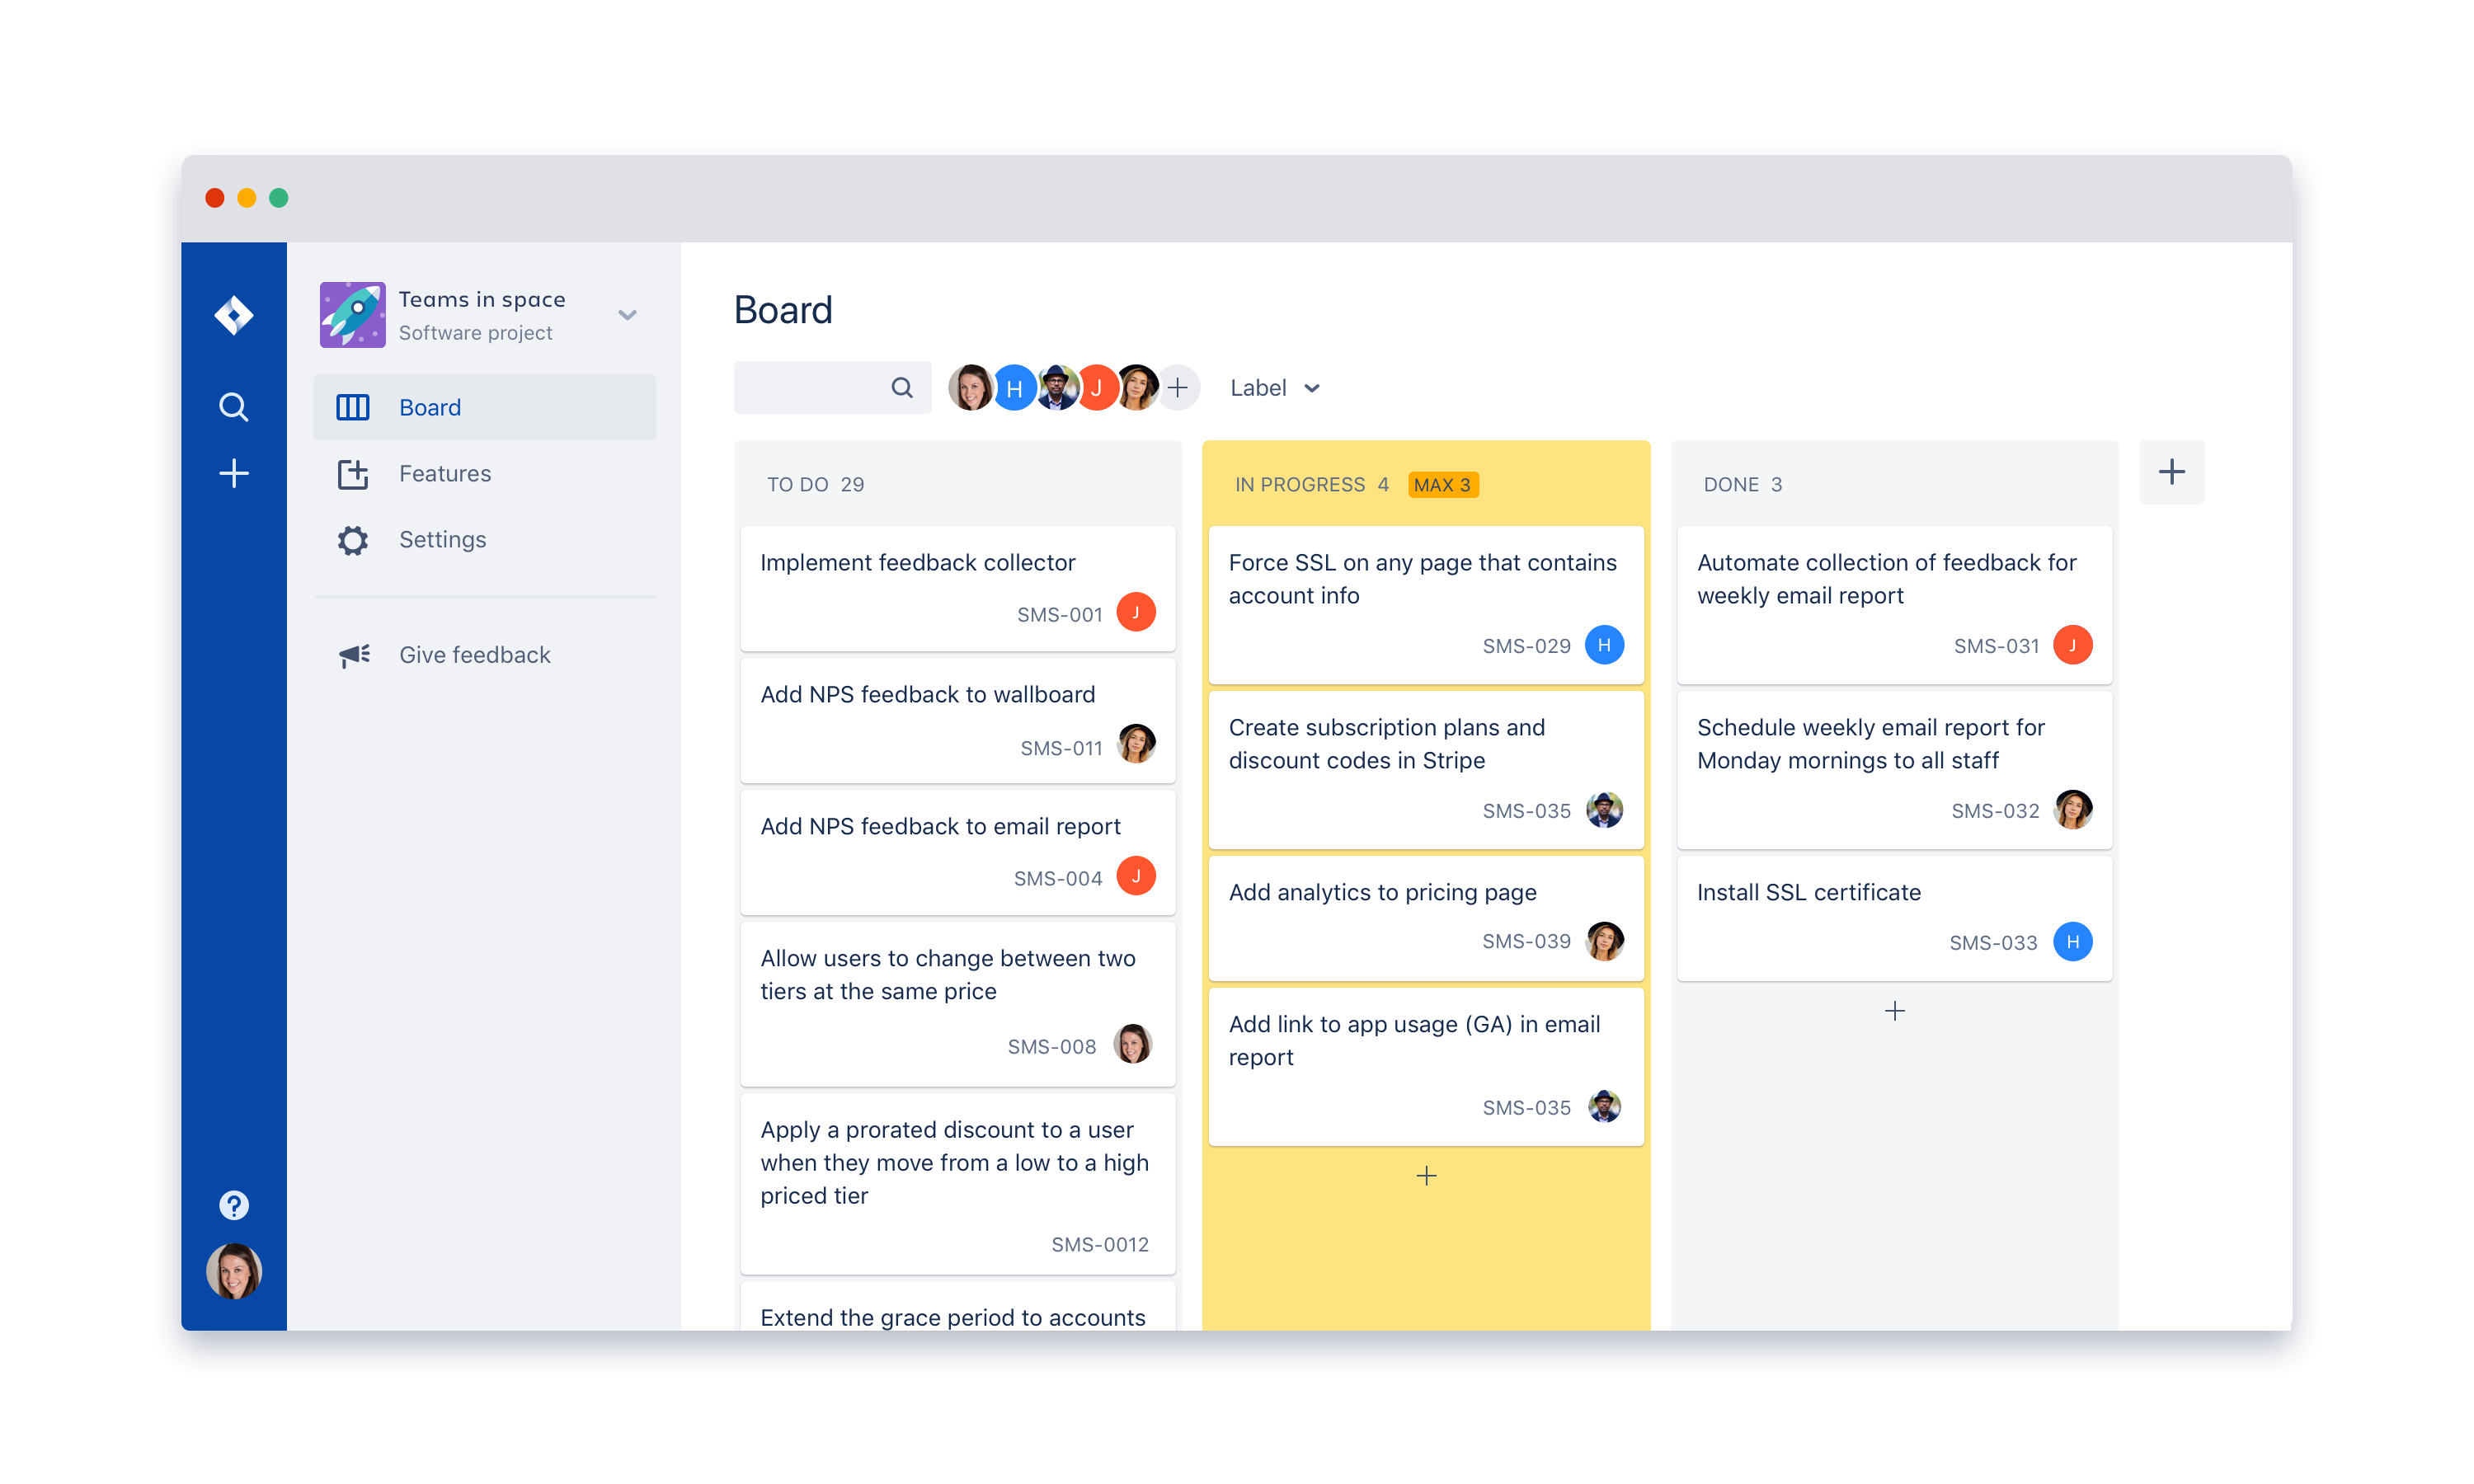
\includegraphics[width=1\textwidth]{Resources/kanban_board_example.png}
	\caption{Beispiel eines Kandan-Boards}
	\label{fig:kanban_board_example}
\end{figure}

Insgesamt bietet Kandan eine einfache und effektive Möglichkeit, den Fortschritt unseres Plotter-Projekts zu verwalten und sicherzustellen, dass wir kontinuierlich Verbesserungen vornehmen und auf unsere Ziele hinarbeiten.

\newpage

\subsection{Anwendung von Kanban}

Im Verlauf unseres Projekts haben wir uns für das Vorgehensmodell Kanban entschieden, um den Entwicklungsprozess zu organisieren und zu steuern. Kanban ist eine agile Methode, die auf kontinuierlicher Verbesserung und Flexibilität basiert. Es hilft, den Arbeitsfluss zu visualisieren, Engpässe zu identifizieren und die Produktivität des Teams zu steigern.

Wir haben ein Kanban-Board verwendet, um unsere Aufgaben und den Fortschritt im Projekt darzustellen. Unser Kanban-Board war in mehrere Spalten unterteilt, die den verschiedenen Phasen des Arbeitsablaufs entsprechen, z.B. 'To Do', 'In Progress', 'Review' und 'Done'. Jede Aufgabe wurde als Karte auf dem Board dargestellt, und wir haben die Karten zwischen den Spalten verschoben, um den Fortschritt der Aufgaben zu visualisieren.

Um den Entwicklungsprozess effektiv zu gestalten, haben wir unser Programm in kleinere Teile aufgeteilt, die wir Vorgänge (in Jira, dem von uns verwendeten Projektmanagement-Tool, genannt) nennen. Dies hat dazu beigetragen, dass wir uns auf bestimmte Aspekte der Anwendung konzentrieren und diese unabhängig voneinander entwickeln konnten.

In regelmäßigen Stand-up-Meetings haben wir den Status unserer Aufgaben überprüft, Engpässe identifiziert und die Prioritäten im Projekt angepasst. Dadurch konnten wir sicherstellen, dass die wichtigsten Aufgaben stets im Fokus standen und effektiv bearbeitet wurden.

\subsection{Vorteile und Erfahrungen}

Durch die Anwendung von Kanban in unserem Projekt haben wir verschiedene Vorteile erfahren:

\begin{itemize}
	\item \textbf{Flexibilität}: Kanban hat es uns ermöglicht, schnell auf Änderungen im Projektumfeld oder in den Anforderungen zu reagieren. Dadurch konnten wir unsere Prioritäten anpassen und sicherstellen, dass wir uns auf die wichtigsten Aspekte des Projekts konzentrierten.
	\item \textbf{Transparenz}: Durch die Visualisierung des Arbeitsablaufs auf dem Kanban-Board konnten alle Teammitglieder den aktuellen Status der Aufgaben und den Fortschritt des Projekts einsehen. Dies hat zu einer besseren Kommunikation und Zusammenarbeit im Team geführt.
	\item \textbf{Effizienz}: Die Anwendung von Kanban und die Aufteilung des Programms in kleinere Vorgänge haben dazu beigetragen, Engpässe im Arbeitsablauf zu identifizieren und zu beseitigen. Dies hat die Produktivität des Teams gesteigert und dazu geführt, dass Aufgaben schneller und effizienter abgeschlossen wurden.
	\item \textbf{Kontinuierliche Verbesserung}: Die regelmäßigen Stand-up-Meetings und die Möglichkeit, den Arbeitsablauf anzupassen, haben dazu beigetragen, kontinuierliche Verbesserungen im Projektprozess zu fördern. Dadurch konnten wir mögliche Probleme frühzeitig erkennen und Lösungen entwickeln, um diese zu beheben.
\end{itemize}

\newpage

Insgesamt hat die Anwendung von Kanban in unserem Projekt dazu beigetragen, einen effizienten und flexiblen Entwicklungsprozess zu gestalten, der es uns ermöglichte, eine erfolgreiche und benutzerfreundliche Anwendung zu entwickeln.

\section{Anforderungsanalyse}
\subsection{Funktionale Anforderungen}
Funktionale Anforderungen beschreiben die Funktionalitäten, die das System bieten soll, um die gewünschten Ziele zu erreichen. Für das Plotter-Projekt umfassen die funktionalen Anforderungen:

\begin{itemize}
	\item Eingabe einer mathematischen Funktion durch den Benutzer.
	\item Grafische Darstellung der eingegebenen Funktion auf einer zweidimensionalen Zeichenfläche.
	\item Verschieben und Zoomen der Zeichenfläche zur besseren Analyse der Funktion.
	\item Hinzufügen und Entfernen von Funktionen.
	\item Möglichkeit zur Bearbeitung der Funktionen, einschließlich Ableitung und Kurvendiskussion.
	\item Verwaltung von Variablen und Konstanten in der Funktion.
	\item Anpassung der Darstellung der Funktion, wie z.B. Farbe und Sichtbarkeit.
\end{itemize}

\subsection{Nicht funktionale Anforderungen}
Nicht funktionale Anforderungen beziehen sich auf die Qualitätsaspekte eines Systems und legen fest, wie gut die funktionalen Anforderungen erfüllt werden. Für das Plotter-Projekt umfassen die nicht funktionalen Anforderungen:

\begin{itemize}
	\item Benutzerfreundlichkeit: Die Anwendung sollte einfach und intuitiv zu bedienen sein.
	\item Leistung: Die Anwendung sollte effizient arbeiten und in angemessener Zeit eine grafische Darstellung der Funktionen erstellen.
	\item Skalierbarkeit: Die Anwendung sollte in der Lage sein, mit einer wachsenden Anzahl von Funktionen und Variablen umzugehen.
	\item Portabilität: Die Anwendung sollte auf verschiedenen Betriebssystemen lauffähig sein.
	\item Zuverlässigkeit: Die Anwendung sollte stabil und fehlerfrei arbeiten.
\end{itemize}

\newpage

\subsection{Aktivitätsdiagramm}
Ein Aktivitätsdiagramm ist eine grafische Darstellung der Arbeitsabläufe und Abläufe innerhalb eines Systems. Es zeigt, wie verschiedene Aktivitäten und Entscheidungen innerhalb des Systems aufeinander folgen und miteinander verknüpft sind.

\begin{figure}[ht]
	\centering
	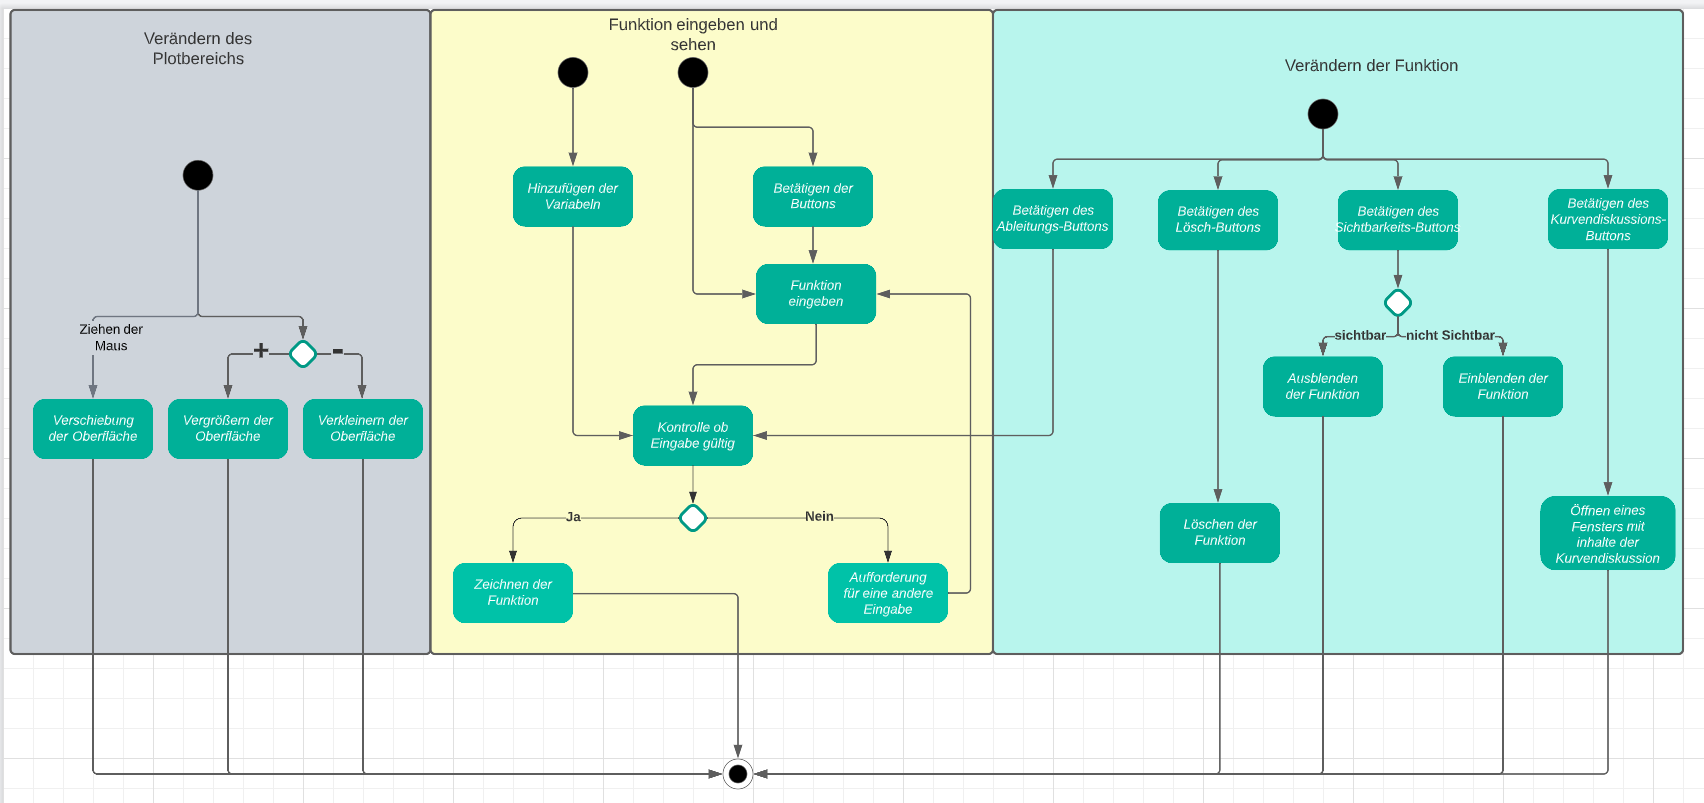
\includegraphics[width=1\textwidth]{Resources/aktivitaetsdiagramm.png}
	\caption{Aktivitätsdiagramm des Plotter-Projekts}
	\label{fig:aktivitaetsdiagramm}
\end{figure}

Das Aktivitätsdiagramm beschreibt den Ablauf eines Plotters. Ein Prozess beginnt damit, dass der Nutzer in ein Textfeld schreiben kann, dies kann er entweder mithilfe von Buttons für Sonderzeichen oder auch direkt. Nachher wird die Eingabe auf ihre Gültigkeit überprüft.
Parallel kann der User auch Variablen hinzufügen, welche auf ihre Gültigkeit anschließend überprüft werden, sollte die Variable falsch eingegeben werden, nimmt es die letzte gültige Eingabe und setzt die Variable auf deren Wert, und gibt gleichzeitig eine Aufforderung aus, dass die Variable richtig eingegeben werden soll. Sollte die Funktion einen falschen Syntax haben, wird wiederum eine Aufforderung angezeigt, welche fordert die Funktion richtig einzugeben. Sollten die Eingaben gültig sein, wird die Funktion gezeichnet.

Wenn der Nutzer die Ansicht des Plottbereichs verändern will, kann er mithilfe des Mausrads zoomen. Zudem kann der User mithilfe von Ziehen der Maus die Oberfläche in x und y Richtung verschieben.
Wenn der Benutzer mit einer vorhandenen Funktion interagieren möchte, kann er die Schaltflächen verwenden. Diese Schaltflächen ermöglichen es ihm, die Funktion auszublenden, wenn sie sichtbar ist, oder sie wieder anzuzeigen, wenn sie ausgeblendet wurde. Außerdem kann er die Funktion löschen, ihre Ableitung berechnen oder sich die vollständige Kurvendiskussion anzeigen lassen.


\newpage

\subsection{Zeiteinteilung}
\begin{table}[h]
	\centering
	\begin{tabular}{|p{5cm}|p{2cm}|p{2cm}|p{2cm}|}
		\hline
		\textbf{Anforderung}                                                                                    & \textbf{Geschätzte Zeit} & \textbf{Priorität (1-10)} & \textbf{Effektive Zeit} \\
		\hline
		Eingegebene mathematische Funktion auf dem Plottbereich anzeigen (Grafisches + Berechnung der Funktion) & 10                       & 10                        & 12                      \\
		\hline
		Mathematische Variablen                                                                                 & 6                        & 8                         & 3                       \\
		\hline
		Zoom im Plottbereich                                                                                    & 3                        & 7                         & 3                       \\
		\hline
		Plottbereich bewegen                                                                                    & 2                        & 7                         & 1+                      \\
		\hline
		Beschriftung der Achsen                                                                                 & 1                        & 8                         & 2                       \\
		\hline
		Ableitungsbutton der Funktion                                                                           & 5                        & 4                         & 2                       \\
		\hline
		Sichtbarkeitsbutton der Funktion                                                                        & 2                        & 5                         & 1                       \\
		\hline
		Löschbutton der Funktion                                                                                & 1                        & 6                         & 1                       \\
		\hline
		Kurvendiskussionsbutton der Funktion                                                                    & 8                        & 3                         & 2                       \\
		\hline
		Styling der Oberfläche                                                                                  & 4                        & 4                         & 5                       \\
		\hline
		Javadocs                                                                                                & 5                        & 8                         & 5                       \\
		\hline
		JUnit                                                                                                   & 6                        & 8 dann 1                  & 6                       \\
		\hline
		Dokumentation des Programms                                                                             & 8                        & 10                        & 20                      \\
		\hline
	\end{tabular}
	\caption{Anforderungsanalyse}
	\label{tab:anforderungsanalyse}
\end{table}

Die Tabelle \ref{tab:anforderungsanalyse} zeigt eine Übersicht über die Anforderungen an das Projekt. Für jede Anforderung wird die geschätzte Zeit für die Implementierung, die Priorität der Anforderung und die tatsächlich aufgewendete Zeit aufgeführt. Es wird deutlich, dass einige Anforderungen, wie die Darstellung der eingegebenen mathematischen Funktion auf dem Plotbereich und die Dokumentation des Programms, eine hohe Priorität hatten und entsprechend mehr Zeit in Anspruch nahmen. Andere Anforderungen, wie der Ableitungsbutton und der Kurvendiskussionsbutton, hatten eine niedrigere Priorität und benötigten weniger Zeit. Insgesamt zeigt die Tabelle, dass die effektive Zeit oft von der geschätzten Zeit abweicht, was auf die Komplexität und die unvorhergesehenen Herausforderungen bei der Implementierung der verschiedenen Anforderungen hinweist.

\newpage

\section{Use-Case-Diagramm}

\subsection{Erklärung}

Das Use-Case-Diagramm beschreibt die Funktionalität des Plotters und zeigt, wie Benutzer mit der Anwendung interagieren können. Der Benutzer kann in ein Textfeld seine gewünschte Funktion eingeben und mithilfe von Buttons Sonderzeichen in das Textfeld schreiben. Der Benutzer hat auch die Möglichkeit, verschiedene Buttons zu verwenden, um die Funktion zu bearbeiten, wie zum Beispiel die Sichtbarkeit, Ableitung, Kurvendiskussion oder die Funktion zu löschen. Zusätzlich kann der Benutzer den Anzeigebereich der Funktion mithilfe von Zoomen oder Verschieben verändern.

\subsection{Diagramm}

Das folgende Diagramm zeigt das Use-Case-Diagramm für unseren Plotter:

\begin{figure}[h]
	\centering
	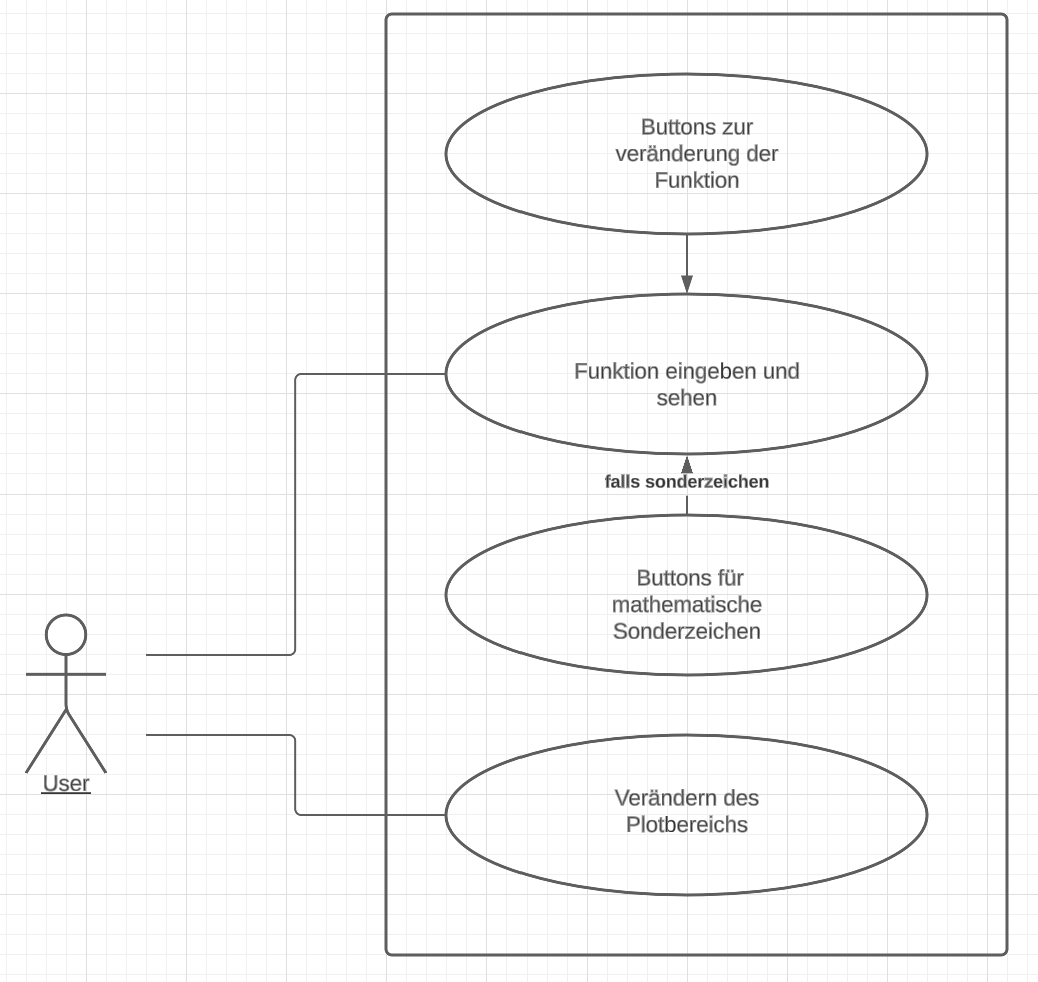
\includegraphics[width=0.8\textwidth]{Resources/use-case-diagram.png}
	\caption{Use-Case-Diagramm des Plotters}
	\label{fig:use_case_diagram}
\end{figure}

Das Diagramm veranschaulicht die verschiedenen Aktionen, die ein Benutzer ausführen kann, um mit der Anwendung zu interagieren und mathematische Funktionen zu visualisieren und zu analysieren.

\section{Systemarchitektur}

\subsection{Übersicht}

Die Systemarchitektur des Projekts ist in zwei Hauptkomponenten unterteilt: das Frontend und das Backend. Das Frontend ist für die Benutzeroberfläche und die Interaktionen mit dem Benutzer verantwortlich, während das Backend die Berechnungen und die Verarbeitung der eingegebenen mathematischen Funktionen übernimmt. Zusammen bieten sie eine effektive und benutzerfreundliche Anwendung zum Plotten von mathematischen Funktionen und ihren Ableitungen.

\subsection{Frontend}

Das Frontend der Anwendung ist mit JavaFX implementiert, einer leistungsstarken und flexiblen Bibliothek für die Erstellung grafischer Benutzeroberflächen. Es bietet eine Vielzahl von UI-Komponenten und Steuerelementen, die für die Implementierung der Anwendung erforderlich sind, einschließlich Szenen, Gruppen, Schaltflächen, Eingabefelder und mehr. Das Frontend ist für die Organisation und Darstellung der Benutzeroberfläche verantwortlich, einschließlich der Eingabefelder für Funktionen, Schaltflächen für mathematische Operationen und Anzeige der Funktionsplots im Plotbereich.

\begin{figure}[h]
	\centering
	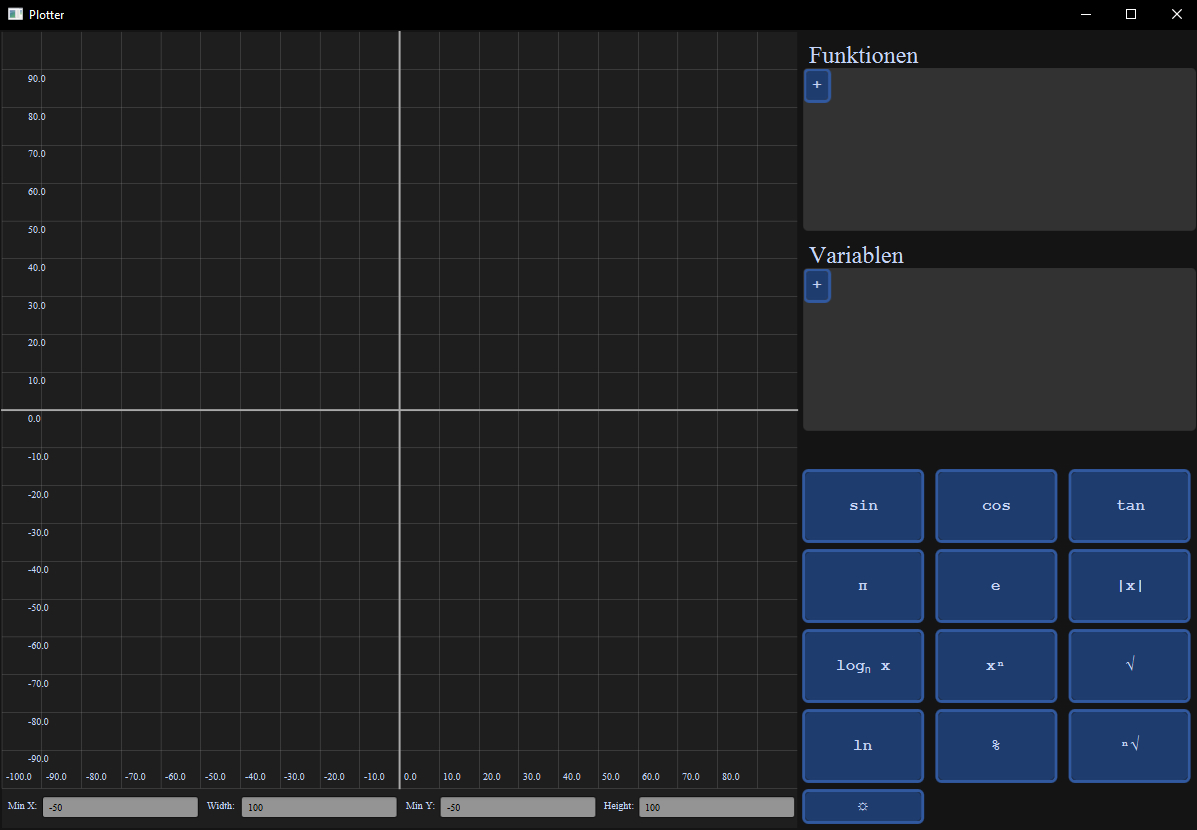
\includegraphics[width=\textwidth]{Resources/gui_screenshot.png}
	\caption{Screenshot der Benutzeroberfläche der Anwendung}
	\label{fig:gui_screenshot}
\end{figure}

\newpage

\subsection{Backend}

Das Backend der Anwendung ist für die Verarbeitung der eingegebenen mathematischen Funktionen, Berechnung der Ableitungen und Aktualisierung des Plotbereichs verantwortlich. Es verwendet die mxparser-Bibliothek, um mathematische Ausdrücke zu parsen und auszuwerten, und die Hauptklassen der Anwendung, um die grafischen Darstellungen der Funktionen und ihrer Ableitungen zu erzeugen. Die Klassen DerivativeCalculator, PlotFunction und PlotArea sind die Hauptkomponenten des Backends und arbeiten zusammen, um die gewünschte Funktionalität bereitzustellen.

\subsection{Klassendiagramm}

Das Klassendiagramm zeigt die Struktur und die Beziehungen zwischen den Hauptklassen der Anwendung. Es hilft dabei, die Verantwortlichkeiten jeder Klasse und die Interaktionen zwischen den Klassen besser zu verstehen.

\begin{itemize}
	\item \textbf{DerivativeCalculator}: Diese Klasse ist verantwortlich für die Berechnung der Ableitungen der eingegebenen mathematischen Funktionen. Sie verwendet die mxparser-Bibliothek und interagiert mit der PlotFunction-Klasse, um die Ableitungen zu berechnen und bereitzustellen.
	\item \textbf{Layout}: Diese Klasse ist ein benutzerdefiniertes JavaFX Group-Objekt, das die Benutzeroberfläche der Anwendung organisiert. Es enthält die Komponenten wie Eingabefelder, Schaltflächen und den Plotbereich und stellt sicher, dass diese Elemente auf dem Bildschirm richtig angeordnet sind.

	\item \textbf{PlotArea}: Diese Klasse ist ein benutzerdefiniertes JavaFX Group-Objekt, das den Plotbereich der Anwendung darstellt. Es verwaltet das Hinzufügen, Entfernen und Aktualisieren von Funktionen, Variablen und Gitterlinien im Plotbereich.

	\item \textbf{PlotFunction}: Die PlotFunction-Klasse verwaltet die grafische Darstellung einer mathematischen Funktion. Sie berechnet die Positionen der Liniensegmente, die die Kurve der Funktion approximieren, und steuert die Sichtbarkeit der Funktion im Plotbereich.

	\item \textbf{Plotter}: Die Plotter-Klasse ist die Hauptklasse der JavaFX-Anwendung und steuert den gesamten Programmablauf. Sie verwendet die mxparser-Bibliothek, um die eingegebenen mathematischen Funktionen zu analysieren und auszuwerten.

	\item \textbf{ScrollPaneFunctionsElement}: Diese Klasse stellt ein einzelnes Funktionselement in der ScrollPane dar, einschließlich eines Textfelds zur Eingabe der Funktion und Schaltflächen zum Berechnen der Ableitung, Löschen der Funktion, Steuern der Sichtbarkeit und Anzeigen der Funktionsanalyse.

	\item \textbf{ScrollPaneVariablesElement}: Diese Klasse stellt ein einzelnes Variablenelement in der ScrollPane dar, einschließlich eines Textfelds zur Eingabe des Variablenwerts und einer Schaltfläche zum Löschen der Variable.
\end{itemize}

Die Klassen interagieren miteinander, um die Hauptfunktionalitäten der Anwendung bereitzustellen. Die Plotter-Klasse agiert als zentraler Koordinator, der die anderen Klassen steuert und verwaltet, um das Plotten von Funktionen, Berechnung von Ableitungen und Aktualisierung der Benutzeroberfläche zu ermöglichen.\\
Im Folgenden finden Sie das Klassendiagramm für das Projekt:

\begin{figure}[h]
	\centering
	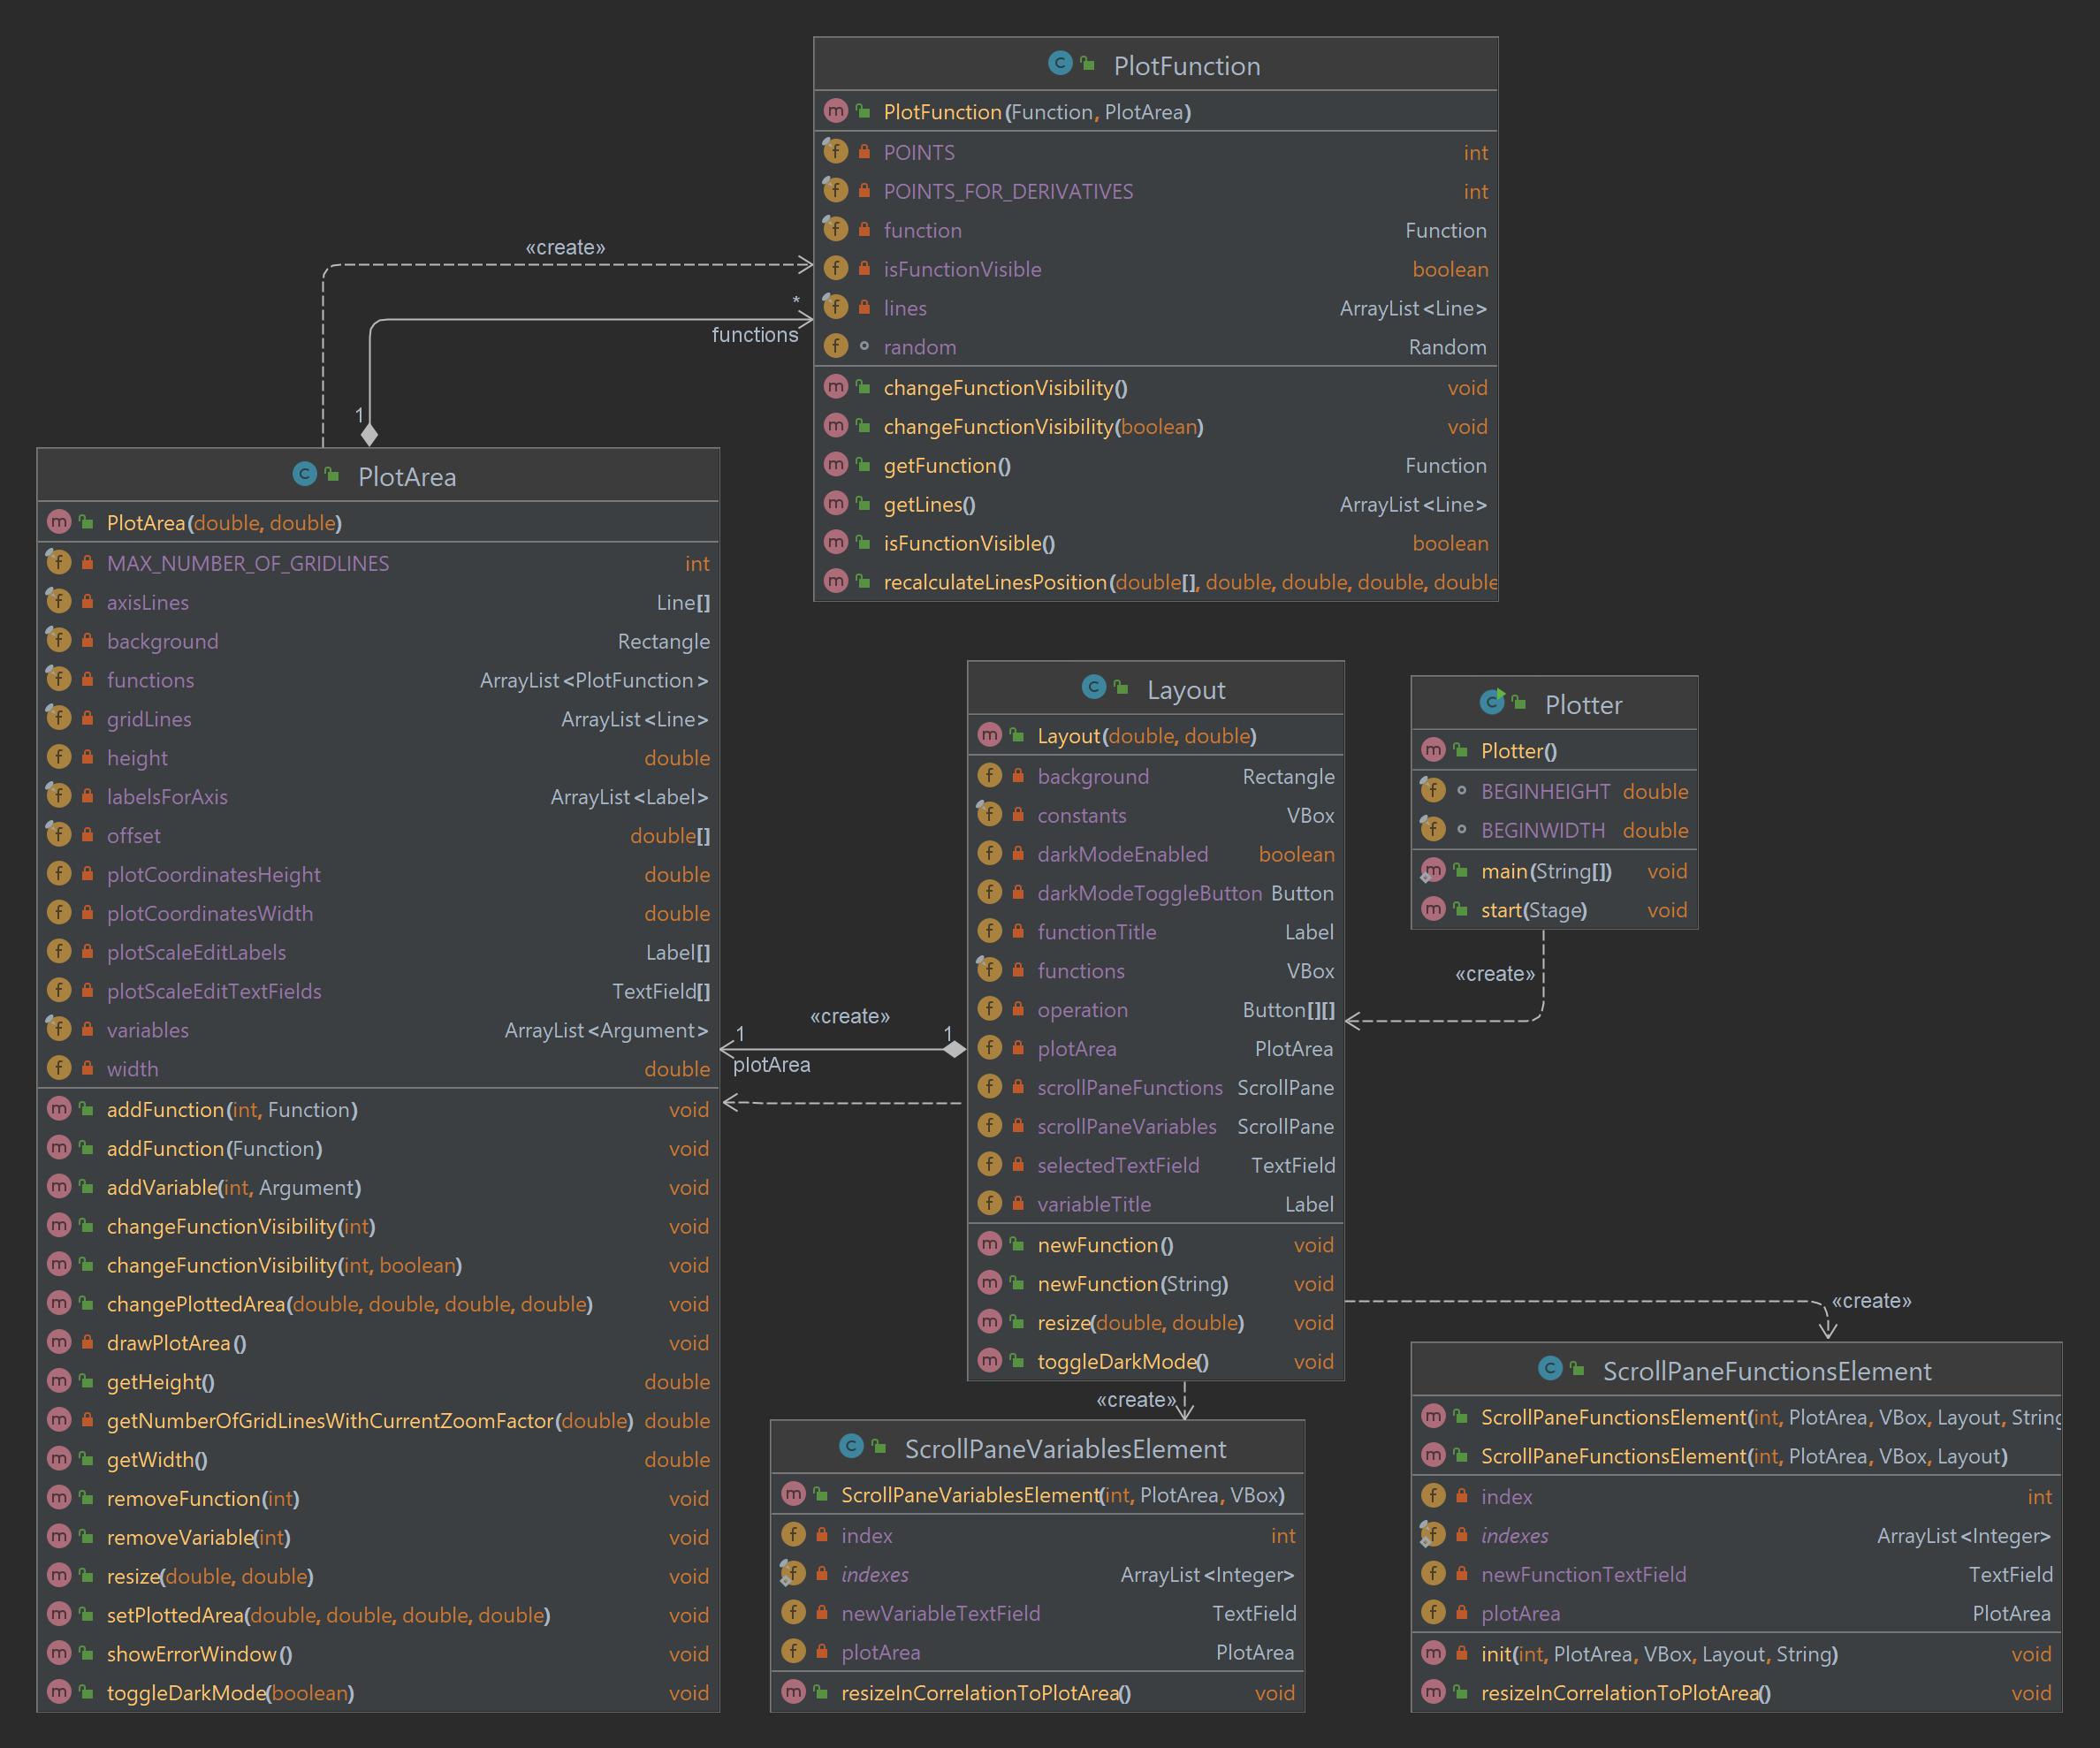
\includegraphics[width=\textwidth]{Resources/class_diagram.png}
	\caption{Klassendiagramm der Hauptklassen}
	\label{fig:class_diagram}
\end{figure}

\newpage

\section{Umsetzung (Programmierung)}

\subsection{UI-Prototyp}

Der UI-Prototyp wurde erstellt, um eine Vorstellung davon zu bekommen, wie die endgültige Benutzeroberfläche aussehen sollte. Dabei orientierte sich das Design optisch am Taschenrechner von Windows. Der Prototyp wurde mithilfe des Figma-Tools erstellt, das eine unkomplizierte und einfache Gestaltung ermöglichte. Die Abbildung \ref{fig:ui_prototype} zeigt den UI-Prototypen. Das Design diente als Basis für die Frontend-Entwicklung und half bei der Entscheidungsfindung für verschiedene Designelemente.

\begin{figure}[ht]
	\centering
	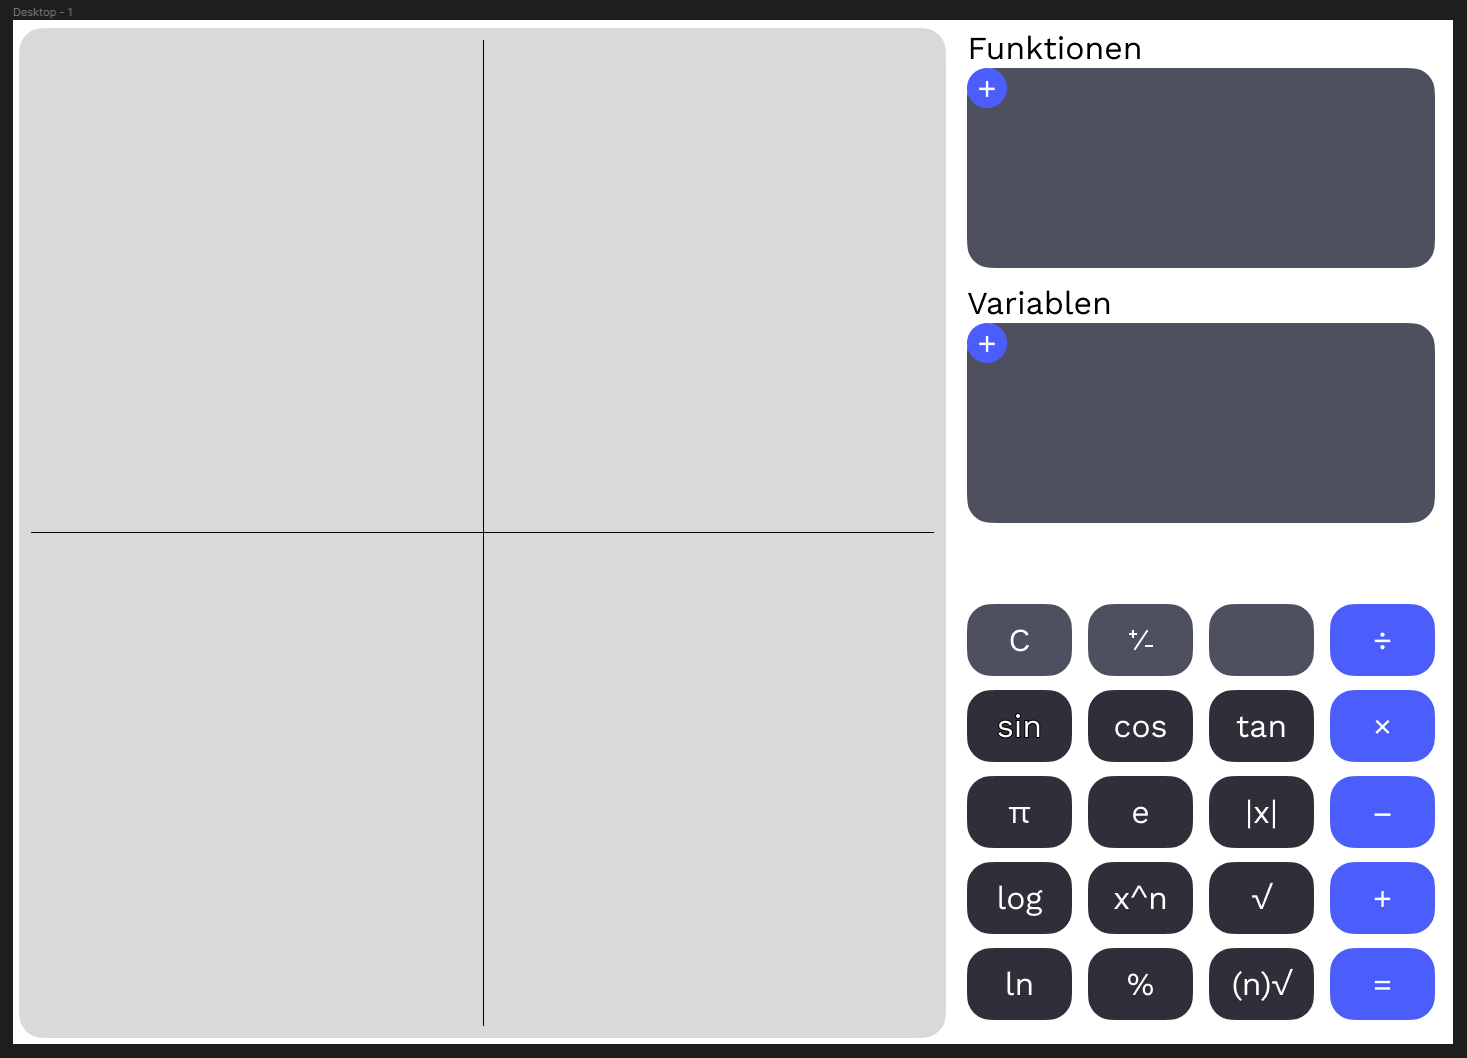
\includegraphics[width=\textwidth]{Resources/ui_prototype.png}
	\caption{UI-Prototyp des Plotters}
	\label{fig:ui_prototype}
\end{figure}

\subsection{Backend-Entwicklung}
Die Backend-Entwicklung fokussierte sich auf die Berechnung von Funktionswerten und Ableitungen sowie die Verarbeitung von Variablen und Konstanten. Eine der größten Herausforderungen bestand darin, die Neuberechnung der einzelnen Punkte des Graphen bei Verschiebung zu optimieren. Dies war besonders wichtig, um die Rechenaufwändigkeit und die Ausführungszeit der Anwendung zu reduzieren. Die Programmierung des Gitternetzes erwies sich ebenfalls als anspruchsvoll. Besonders das Verschieben des Gitters und das korrekte Darstellen der Funktion bei veränderter Skalierung und Positionierung erforderten eine präzise Koordination der Berechnungen.

\subsection{Frontend-Entwicklung}
Die Frontend-Entwicklung konzentrierte sich auf die Gestaltung der Benutzeroberfläche und die Implementierung der verschiedenen UI-Komponenten. Insbesondere die Erstellung und Formatierung der Knöpfe für die Eingabe von Funktionen, Variablen und mathematischen Operationen stellte eine Herausforderung dar. Die Verwendung von HTML, CSS und JavaFX für das Styling und Layout der Benutzeroberfläche erleichterte den Prozess. Dennoch war es schwierig, alle Elemente so zu gestalten, dass sie korrekt miteinander interagierten, insbesondere beim Verschieben des Netzwerks oder beim Anpassen der Größe des gesamten Fensters. Das Erstellen von Rändern und optisch ansprechenden Knöpfen erforderte ebenfalls besondere Aufmerksamkeit.

\subsection{Integration von APIs}
Die mxParser-Bibliothek wurde für die Berechnung von mathematischen Funktionen und deren Ableitungen ausgewählt und in das Projekt integriert. Die Bibliothek zeichnet sich durch ihre umfangreichen Möglichkeiten und gute Dokumentation aus, die den Entwicklungsprozess erheblich erleichterten. Die Integration verlief problemlos und fehlerfrei. Die Anwendung nutzt mxParser für das Parsen und Evaluieren der eingegebenen Funktionen, um deren Graphen darzustellen.

\subsection{Teststrategie}
Um die Qualität und Korrektheit der implementierten Funktionen zu gewährleisten, wurde eine Teststrategie entwickelt und JUnit-Tests für verschiedene Aspekte der Anwendung erstellt. Es wurden verschiedene Arten von Funktionen getestet, wie beispielsweise lineare, quadratische und höhergradige Funktionen. Die Tests verglichen die berechneten Werte der Anwendung mit den tatsächlichen Werten und stellten sicher, dass die Abweichungen innerhalb eines akzeptablen Bereichs lagen (in der Regel auf drei Nachkommastellen genau).

Gelegentlich kam es zu geringfügigen Abweichungen in den Ergebnissen, die jedoch auf die Unvermeidlichkeit von Rundungsfehlern und die Begrenzungen von Java bei der Verarbeitung von Gleitkommazahlen zurückzuführen sind. Beispielsweise kann es vorkommen, dass statt dem Wert 3,0 der Wert 3,000000000003 errechnet wird. Diese Abweichungen sind jedoch für die Zwecke der Anwendung vernachlässigbar und beeinträchtigen nicht die Funktionalität des Plotters.

\newpage

\section{Benutzung (User Guide)}

\subsection{Installation und Einrichtung}
Um die Plotter-Anwendung zu installieren und einzurichten, befolgen Sie die folgenden Schritte:

\begin{enumerate}
	\item Stellen Sie sicher, dass JDK 11 oder höher und JavaFX 11 oder höher auf Ihrem Computer installiert sind.
	\item Klone das Projekt-Repository von GitHub:\\
	      \texttt{git clone https://github.com/TheD4rkCoder/Plotter}\\
	      \texttt{cd plotter}
	\item Erstellen Sie das Projekt mit Maven:\\
	      \texttt{mvn clean install}
	\item Führen Sie die Anwendung aus:\\
	      \texttt{java --module-path /path/to/javafx-sdk-11/lib\\ --add-modules javafx.controls,javafx.fxml -jar target/plotter-1.0-SNAPSHOT.jar}\\
	      Ersetzen Sie dabei \texttt{/path/to/javafx-sdk-11/lib} durch den Pfad zum JavaFX SDK \texttt{lib}-Verzeichnis.
\end{enumerate}

\subsection{Bedienung der Anwendung}
\begin{enumerate}
	\item Geben Sie eine Funktion in das Textfeld ein und drücken Sie Enter. Die Funktion wird dem Graphen hinzugefügt.
	      \begin{figure}[ht]
		      \centering
		      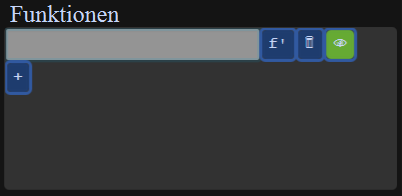
\includegraphics[width=0.7\textwidth]{Resources/example_function.png}
		      \caption{Eingabefeld Funktion}
		      \label{fig:example_function}
	      \end{figure}
	      \newpage
	\item Klicken Sie auf die Schaltflächen neben der Funktion, um verschiedene Aktionen auszuführen:
	      \begin{itemize}
		      \item f': Berechnen und Anzeigen der Ableitung der Funktion
		      \item \(\mathrm{\large{\textbf{X}}}\): Entfernen der Funktion aus dem Graphen
		      \item \(\mathrm{\large{\textbf{O}}}\): Umschalten der Sichtbarkeit der Funktion im Graphen
	      \end{itemize}
	      \begin{figure}[ht]
		      \centering
		      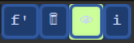
\includegraphics[width=0.5\textwidth]{Resources/example_buttons.png}
		      \caption{Funktionsschaltflächen}
		      \label{fig:example_buttons}
	      \end{figure}
\end{enumerate}

\subsection{Beispiele}
Folgende Beispiele zeigen verschiedene Funktionen, die mit dem Plotter dargestellt werden können:

\begin{enumerate}
	\item Lineare Funktion: \(y = 2x + 1\)
	      \begin{figure}[ht]
		      \centering
		      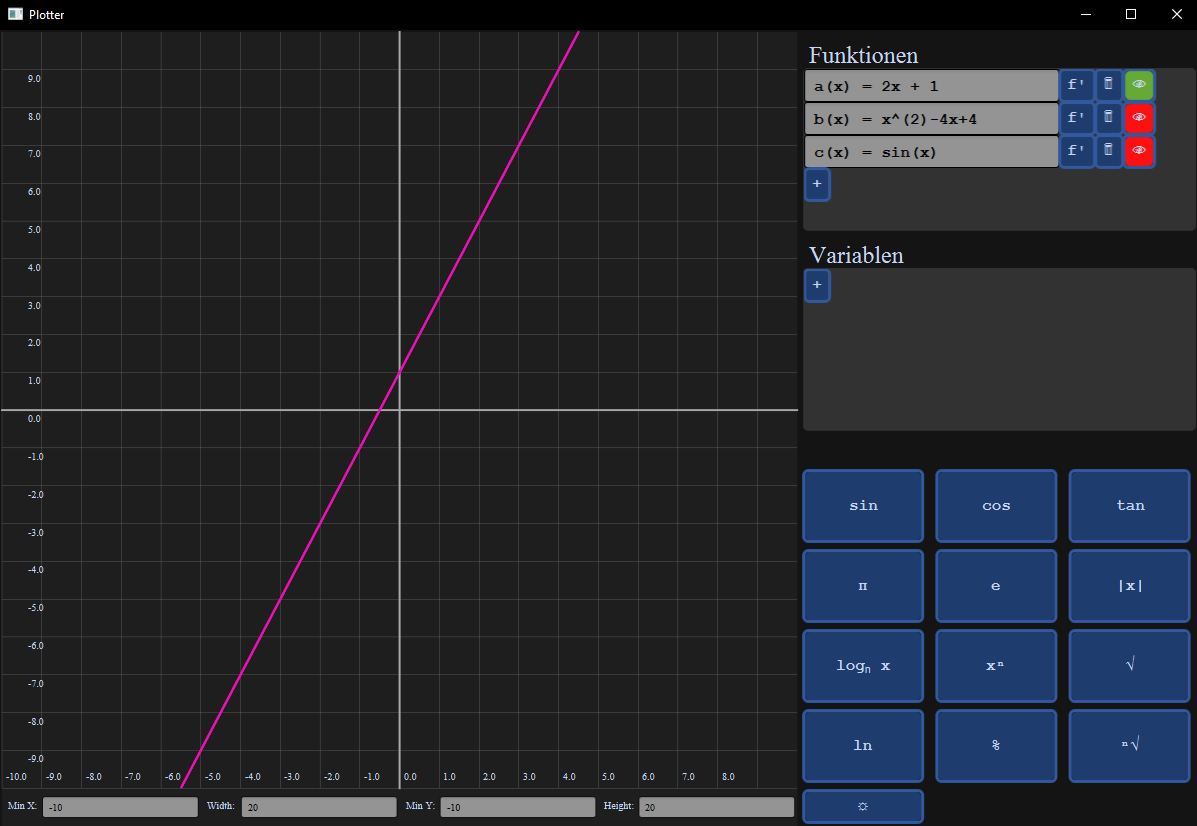
\includegraphics[width=0.8\textwidth]{Resources/example_linear.png}
		      \caption{Lineare Funktion}
		      \label{fig:example_linear}
	      \end{figure}
	      \newpage
	\item Quadratische Funktion: \(y = x^2 - 4x + 4\)
	      \begin{figure}[ht]
		      \centering
		      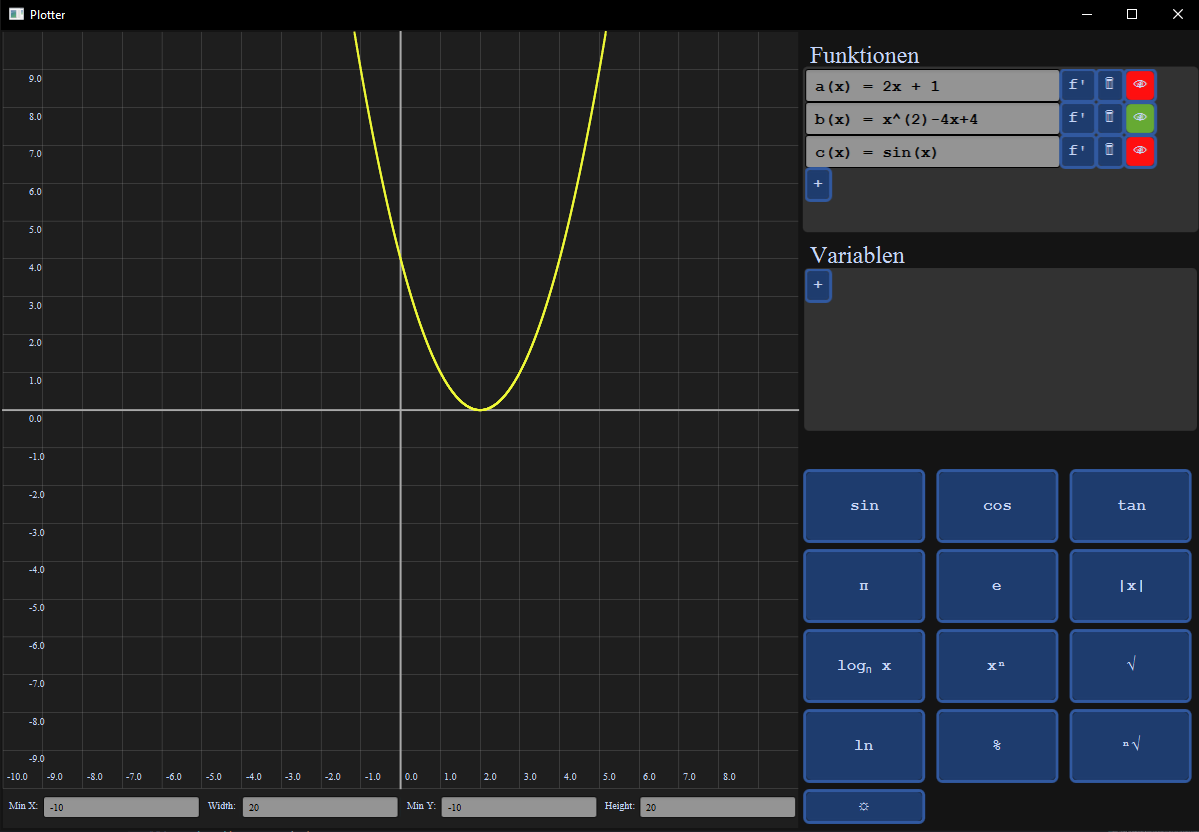
\includegraphics[width=0.8\textwidth]{Resources/example_quadratic.png}
		      \caption{Quadratische Funktion}
		      \label{fig:example_quadratic}
	      \end{figure}
	\item Trigonometrische Funktion: \(y = \sin(x)\)
	      \begin{figure}[ht]
		      \centering
		      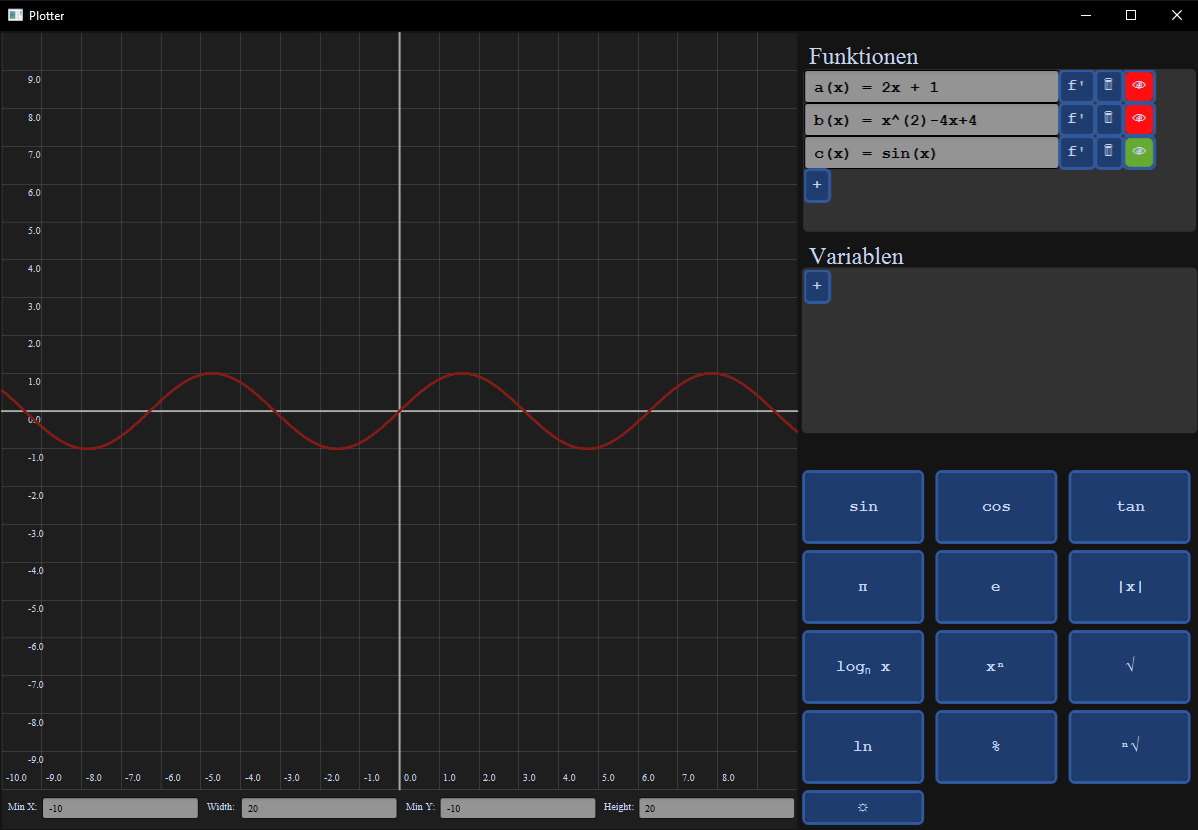
\includegraphics[width=0.8\textwidth]{Resources/example_trigonometric.png}
		      \caption{Trigonometrische Funktion}
		      \label{fig:example_trigonometric}
	      \end{figure}
\end{enumerate}

\newpage

\section{Fazit}

\subsection{Zusammenfassung}
In diesem Projekt haben wir erfolgreich eine Java-basierte Plotter-Anwendung entwickelt, die es Benutzern ermöglicht, mathematische Funktionen und ihre Ableitungen grafisch darzustellen. Wir haben das flexible und leicht verständliche Kanban-System zur Verwaltung unserer Arbeitsabläufe verwendet. Durch den Einsatz von APIs wie mxParser und JavaFX haben wir eine effiziente und benutzerfreundliche Anwendung erstellt, die eine breite Palette von Funktionen unterstützt.

\subsection{Erreichte Ziele}
Die wichtigsten erreichten Ziele sind:
\begin{itemize}
	\item Erstellung einer benutzerfreundlichen grafischen Benutzeroberfläche.
	\item Implementierung von Funktionen zum Hinzufügen, Entfernen und Anzeigen von Funktionen und deren Ableitungen.
	\item Bereitstellung von Funktionen zur Anpassung der Darstellung des Plottbereichs und zum Zoomen.
	\item Erfolgreiche Integration externer APIs und Bibliotheken, wie mxParser und JavaFX, zur Verbesserung der Anwendung.
\end{itemize}

\subsection{Zukünftige Erweiterungen}
Mögliche zukünftige Erweiterungen der Plotter-Anwendung könnten sein:
\begin{itemize}
	\item Hinzufügen weiterer Funktionstypen, wie parametrische und Polarkurven.
	\item Implementierung von Funktionen zur Analyse von Funktionen, wie Nullstellen, Extremwerte und Wendepunkte.
	\item Verbesserung der Leistung und Effizienz der Anwendung, insbesondere bei der Darstellung komplexer Funktionen und bei der Interaktion mit dem Plottbereich.
	\item Erweiterung der Anwendung um 3D-Plotting-Funktionen, um dreidimensionale Funktionen und Oberflächen darzustellen.
\end{itemize}

\newpage

\section{Anhang}

\subsection{Arbeitstagebuch (Planung)}
\begin{table}[h]
	\centering
	\begin{tabularx}{\textwidth}{>{\hsize=0.5\hsize}X>{\hsize=0.5\hsize}X>{\hsize=0.3\hsize}X>{\hsize=2.7\hsize}X}
		\toprule
		\textbf{Person} & \textbf{Datum} & \textbf{Zeit} & \textbf{Tätigkeiten}                                             \\
		\midrule
		Daniel          & 16.01.         & 1h            & Auf github registriert, Beginn Use-Case                          \\
		David           & 16.01.         & 1h            & Erstellung des Git-Repositorys, Besprechung des Projekts         \\
		Patrick         & 16.01.         & 1h            & Erstellung Jira Projekt, Beginn Erstellung UseCaseDiagram(Lucid) \\
		Daniel          & 30.01          & 1h            & Fertigstellung Use-Case Diagramm                                 \\
		David           & 30.01          & 1h            & helfen beim Use-Case Diagramm                                    \\
		David           & 06.02.         & 1h            & Schauen, wie ein Aktivitätsdiagramm und Ablaufdiagramm aussieht  \\
		David           & 12.02.         & 1h            & Anforderungsanalyse                                              \\
		\bottomrule
	\end{tabularx}
	\caption{Planung}
	\label{table:planung}
\end{table}

\subsection{Arbeitstagebuch (Umsetzung)}
\begin{table}[h]
	\centering
	\begin{tabularx}{\textwidth}{>{\hsize=0.5\hsize}X>{\hsize=0.5\hsize}X>{\hsize=0.3\hsize}X>{\hsize=2.7\hsize}X}
		\toprule
		\textbf{Person} & \textbf{Datum} & \textbf{Zeit} & \textbf{Tätigkeiten}                                                                                                                                                                         \\
		\midrule
		alle            & 17.04.         & 3h            & Tests schreiben (für Ableitung, Klasse Plotarea und sonstige Konstanten und mathematische Funktionen wie Sinus)                                                                              \\
		David           & 19.04.         & 4h            & zeichnen der PlotFunction in PlotArea                                                                                                                                                        \\
		David           & 26.04          & 3h            & PlotArea changePlottedArea und drawPlotArea Methoden                                                                                                                                         \\
		David           & 30.04          & 4h            & Menü für die eingabe von Funktionen, Konstanten und Knöpfe für mathematische Funktionen sowie Knöpfe zur löschung, ableitung und umstellen der Sichtbarkeit einer Funktion. Auch Css styling \\
		Patrick         & 20.05.         & 1h            & updated README.md                                                                                                                                                                            \\
		David           & 20.05.         & 1h            & Kommentieren                                                                                                                                                                                 \\
		\bottomrule
	\end{tabularx}
	\caption{Umsetzung}
	\label{table:umsetzung}
\end{table}

\subsection{Quellcode}
Der Quellcode für das Plotter-Projekt ist auf GitHub verfügbar:
\url{https://github.com/TheD4rkCoder/Plotter/tree/master/src/main/java/com/example/plotter}

\subsection{Anwendungsdiagramm}


\clearpage

\subsection{Screenshots}
Folgende Screenshots können in den Anhang aufgenommen werden:
\begin{figure}[ht]
	\centering
	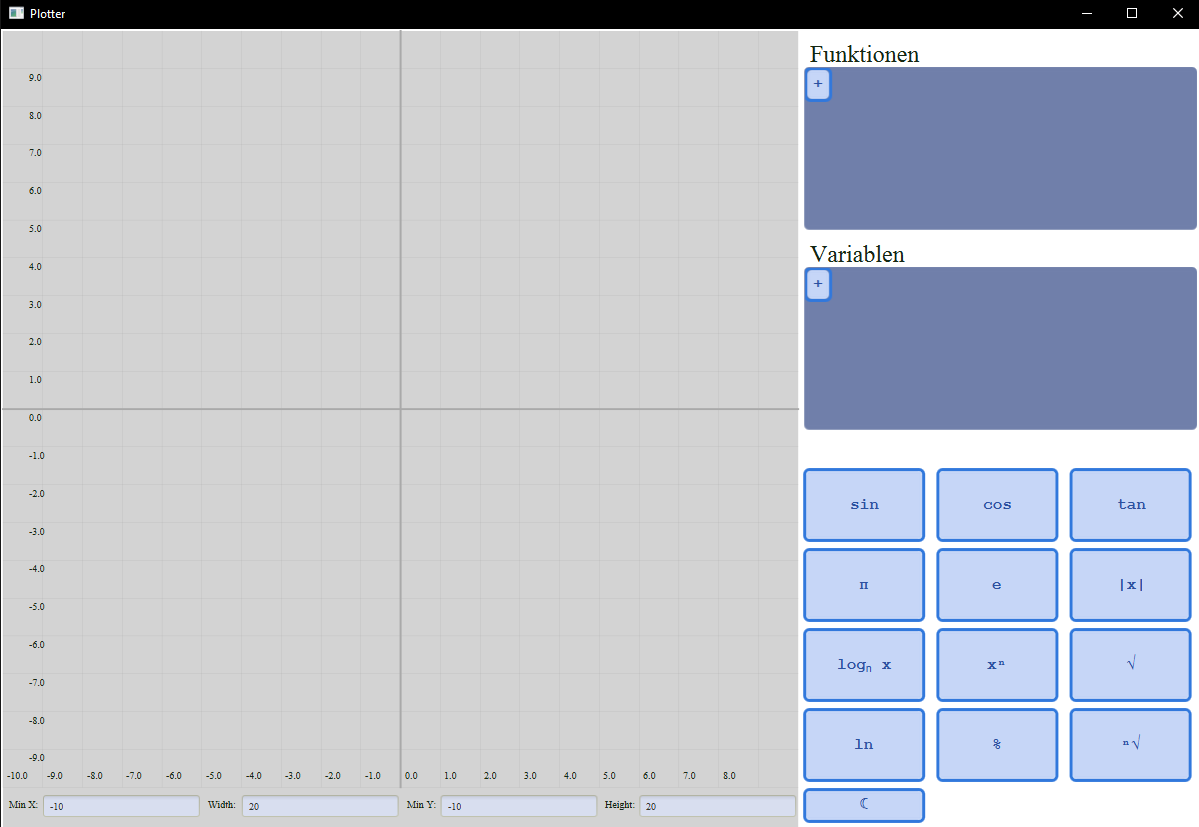
\includegraphics[width=0.8\textwidth]{Resources/startbildschirm.png}
	\caption{Startbildschirm: Leer, ohne Funktionen, im weißen Modus}
	\label{fig:startbildschirm}
\end{figure}

\begin{figure}[ht]
	\centering
	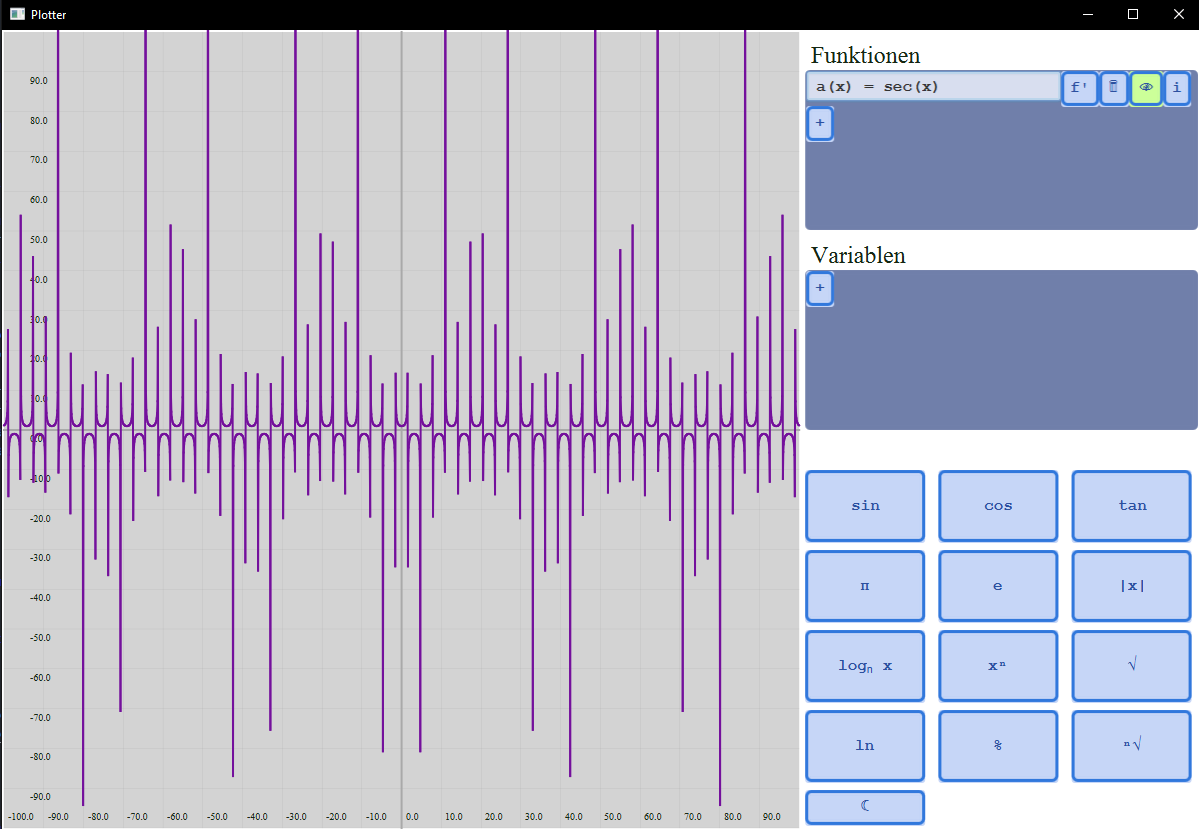
\includegraphics[width=0.8\textwidth]{Resources/eingabe_darstellung.png}
	\caption{Eingabe und Darstellung der Funktion $sec(x)$}
	\label{fig:eingabe_darstellung}
\end{figure}

\begin{figure}[ht]
	\centering
	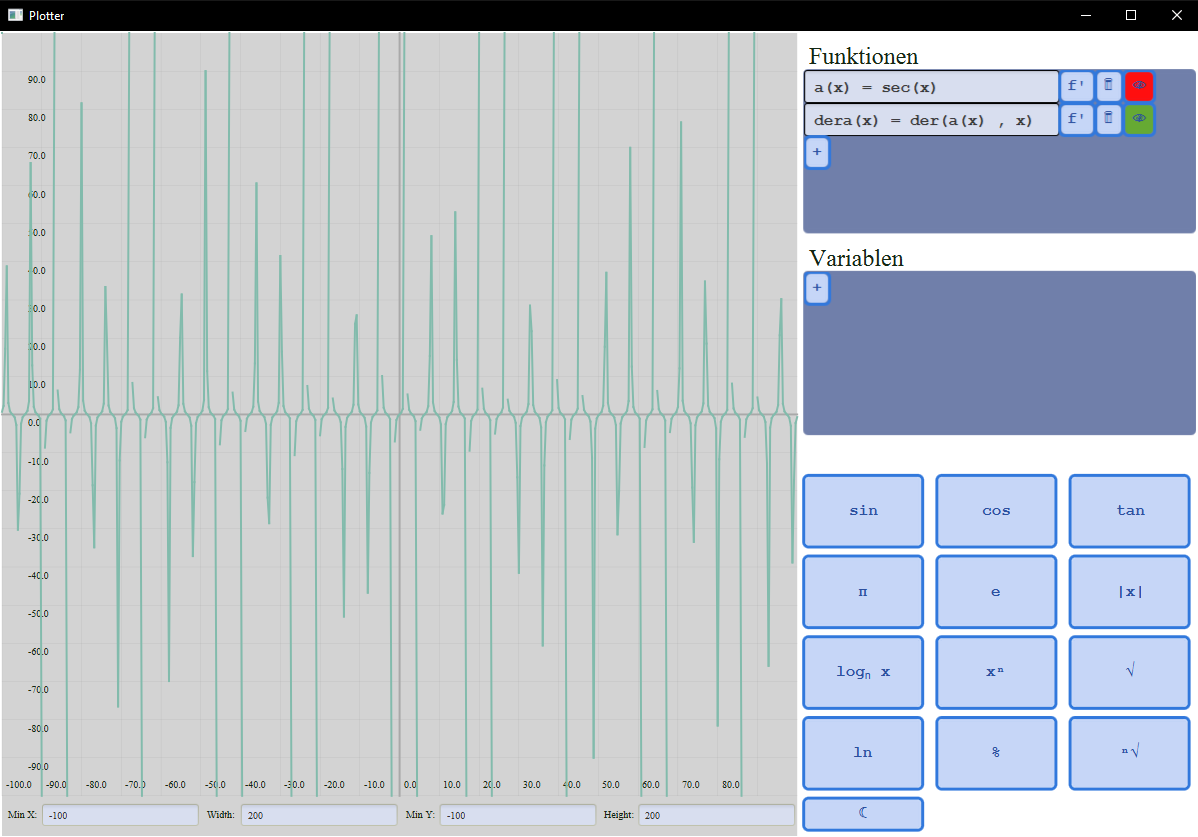
\includegraphics[width=0.8\textwidth]{Resources/anwendung.png}
	\caption{Ableitung der $sec(x)$ Funktion und Ausblenden}
	\label{fig:anwendung}
\end{figure}

\begin{figure}[ht]
	\centering
	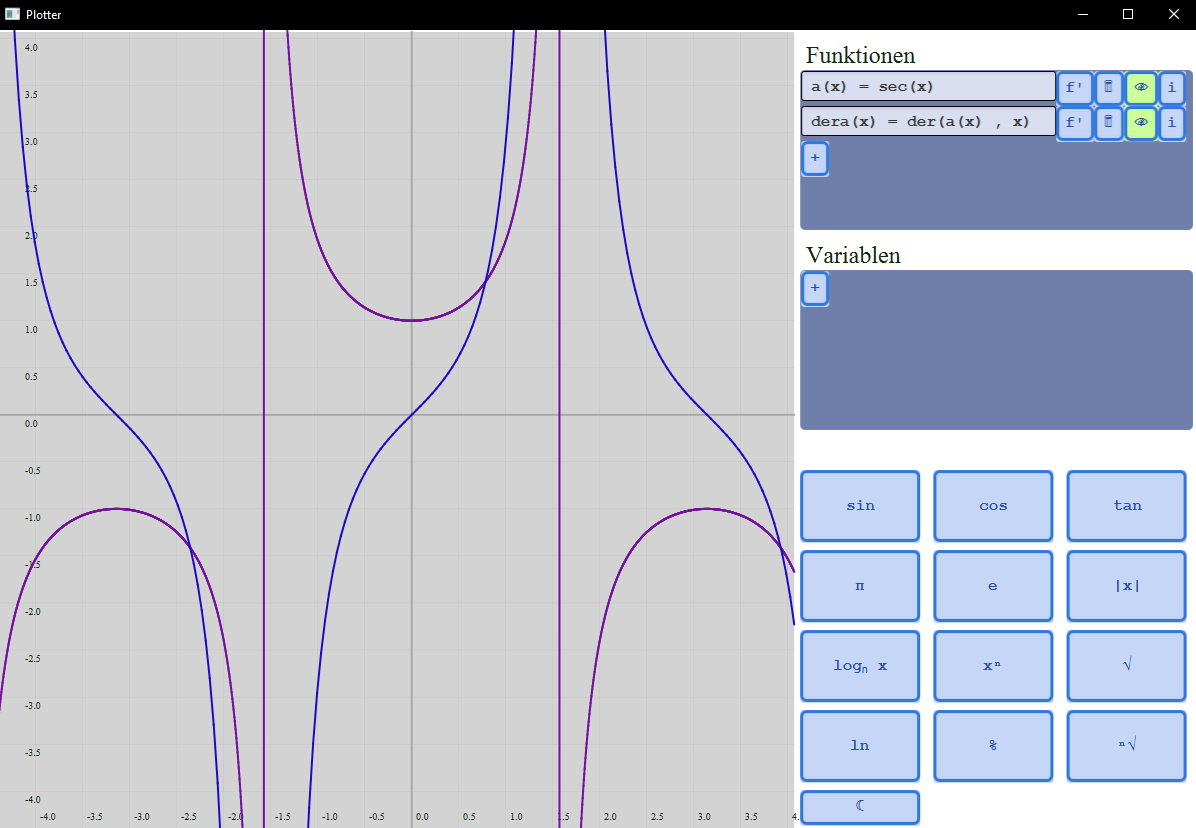
\includegraphics[width=0.8\textwidth]{Resources/zoom.png}
	\caption{Zoom: Gezoomte Ansicht der $sec(x)$ Funktion}
	\label{fig:zoom}
\end{figure}

\begin{figure}[ht]
	\centering
	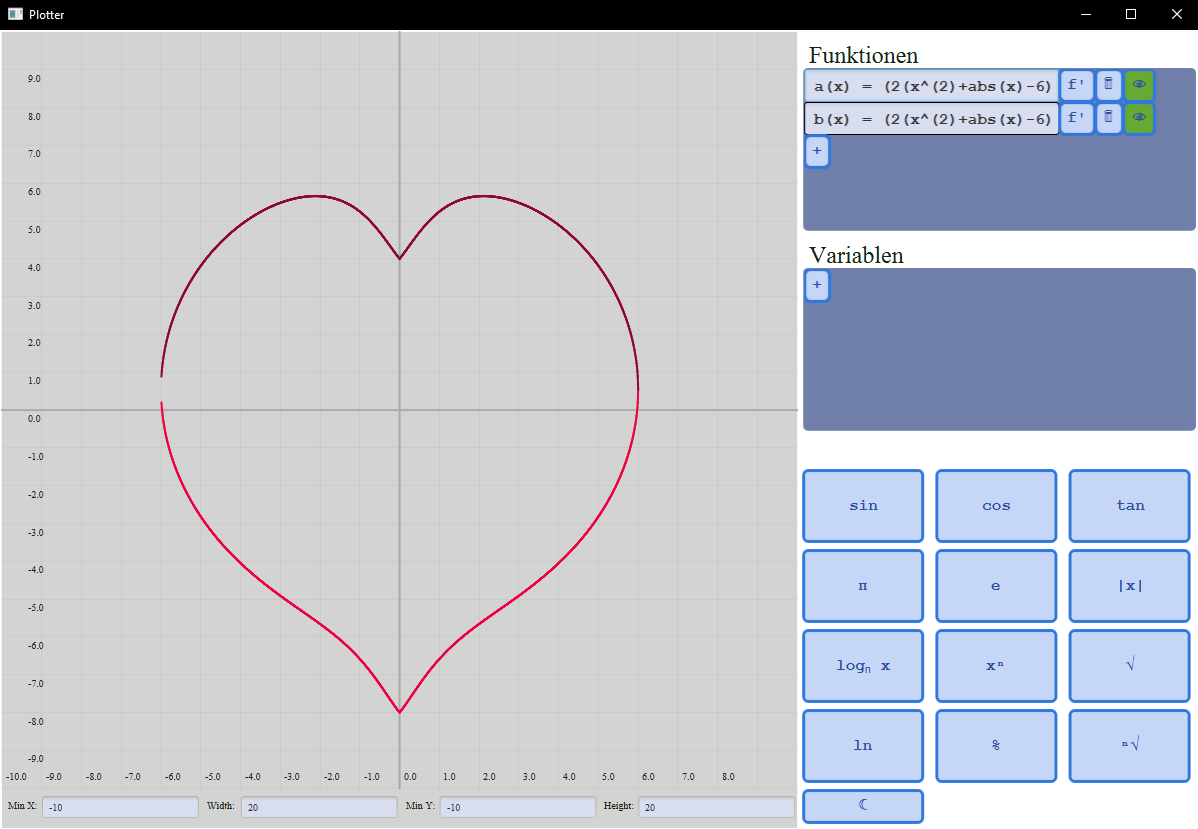
\includegraphics[width=0.8\textwidth]{Resources/heartshape.png}
	\caption{Funktion in der Form eines Herzens}
	\label{fig:heart}
\end{figure}

\clearpage

\subsection{Lizenzinformationen}
Dieses Projekt steht unter der MIT-Lizenz, die eine permissive Open-Source-Lizenz ist. Die MIT-Lizenz ermöglicht die uneingeschränkte Nutzung, Kopie, Modifikation und Weiterverteilung des Projekts, solange die Lizenzbestimmungen eingehalten werden.

Die MIT-Lizenz hat folgende Bedingungen:

\begin{enumerate}
	\item Die Urheberrechts- und Lizenzinformationen müssen in allen Kopien oder wesentlichen Teilen des Projekts enthalten sein.
	\item Die Software wird ``wie sie ist'' bereitgestellt, ohne jegliche ausdrückliche oder stillschweigende Garantie, einschließlich, aber nicht beschränkt auf, die Garantie der Marktgängigkeit, der Eignung für einen bestimmten Zweck und der Nichtverletzung von Schutzrechten.
	\item In keinem Fall haften die Autoren oder Inhaber von Urheberrechten für Schäden oder sonstige Haftungsansprüche, die sich aus oder im Zusammenhang mit der Software oder deren Verwendung oder anderem Handeln mit der Software ergeben.
\end{enumerate}

Für weitere Informationen zur MIT-Lizenz können Sie auf folgenden Link verweisen: \url{https://opensource.org/licenses/MIT}

Durch die Verwendung der MIT-Lizenz wird sichergestellt, dass das Projekt frei zugänglich ist und von anderen Entwicklern zur Zusammenarbeit, Verbesserung und Erweiterung des Projekts verwendet werden kann.

\newpage

\subsection{Abbildungsverzeichnis}
\listoffigures


\end{document}